% talk with nice pictures /mnt/backup/safe-with-time/torben/safed/0321/talk/talk.lisp  amazingly i wrote this presentation in lisp!
% theory /mnt/backup/safe-with-time/torben/safed/0417
% WP6 D6.6 Report on DIC experiments /mnt/backup/safe-with-time/torben/safed/1125
\chapter{DIC}
\lstdefinelanguage{Maxima}{
keywords={addrow,addcol,zeromatrix,ident,augcoefmatrix,ratsubst,diff,ev,tex,%
with_stdout,nouns,express,depends,load,submatrix,div,grad,curl,%
rootscontract,solve,part,assume,sqrt,integrate,abs,inf,exp},
sensitive=true,
comment=[n][\itshape]{/*}{*/}
}
\lstset{language=Maxima}

\citep{Schwertner2008}


\section{Introduction}
In our project we have the task to convert the light field coming from
the micro-mirror array, which acts a pure phase device, into a spatial
intensity distribution. One way to do this is to use a Fourier filter
that rejects light from tilted micro-mirrors. This is the method that
we decided to implement for the project. It is called Schlieren
optical system in documents by our partner In-Vision. However, this
method has the limitation that the solid angle of the illumination
rays must be confined by the diffraction angle (given by the pixel
pitch of $\unit[16]{\mu m}$ of the micro-mirrors). In other words: the
illumination light must exhibit a certain spatial coherence. In our
application this eventually \emph{limits the field of view} of the
microscope. The DIC method that is investigated in this report is a
completely different approach to convert the phase device into an
intensity device and doesn't come with the same limitations as the
Fourier filtering approach. It is possible to get a high contrast even
for a large angular spread of incoherent illumination.

This report documents the second iteration of experiments
investigating the differential interference contrast (DIC) method. A
completely new experimental setup was used (see \figref{fig:dic_mma}
for diagram and \figref{fig:dic_photo} for photo). This was necessary
because optical image quality seems to have a strong impact on the
contrast measurements. Therefore in the new setup we use achromatic
doublets for the two most important imaging lenses.
\begin{figure}[ht]
  \centering
  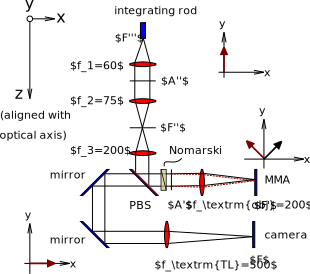
\includegraphics[height=8cm]{../app_dic/img/dic_mma}
  \caption{ Schematic of the optical setup. Apertures allow control of
    the illumination in the planes $A''$ and $F''$. The wire grid
    polarising beam splitter (PBS) is oriented with the aluminium
    coated side towards the Nomarski prism. The Nomarski prism can be
    rotated around the optical axis. The DIC method only works for
    $\pm 45^\circ$ and $\pm 135^\circ$ settings. }
  \label{fig:dic_mma}
\end{figure}
\newpage
\begin{figure}[ht]
  \centering
  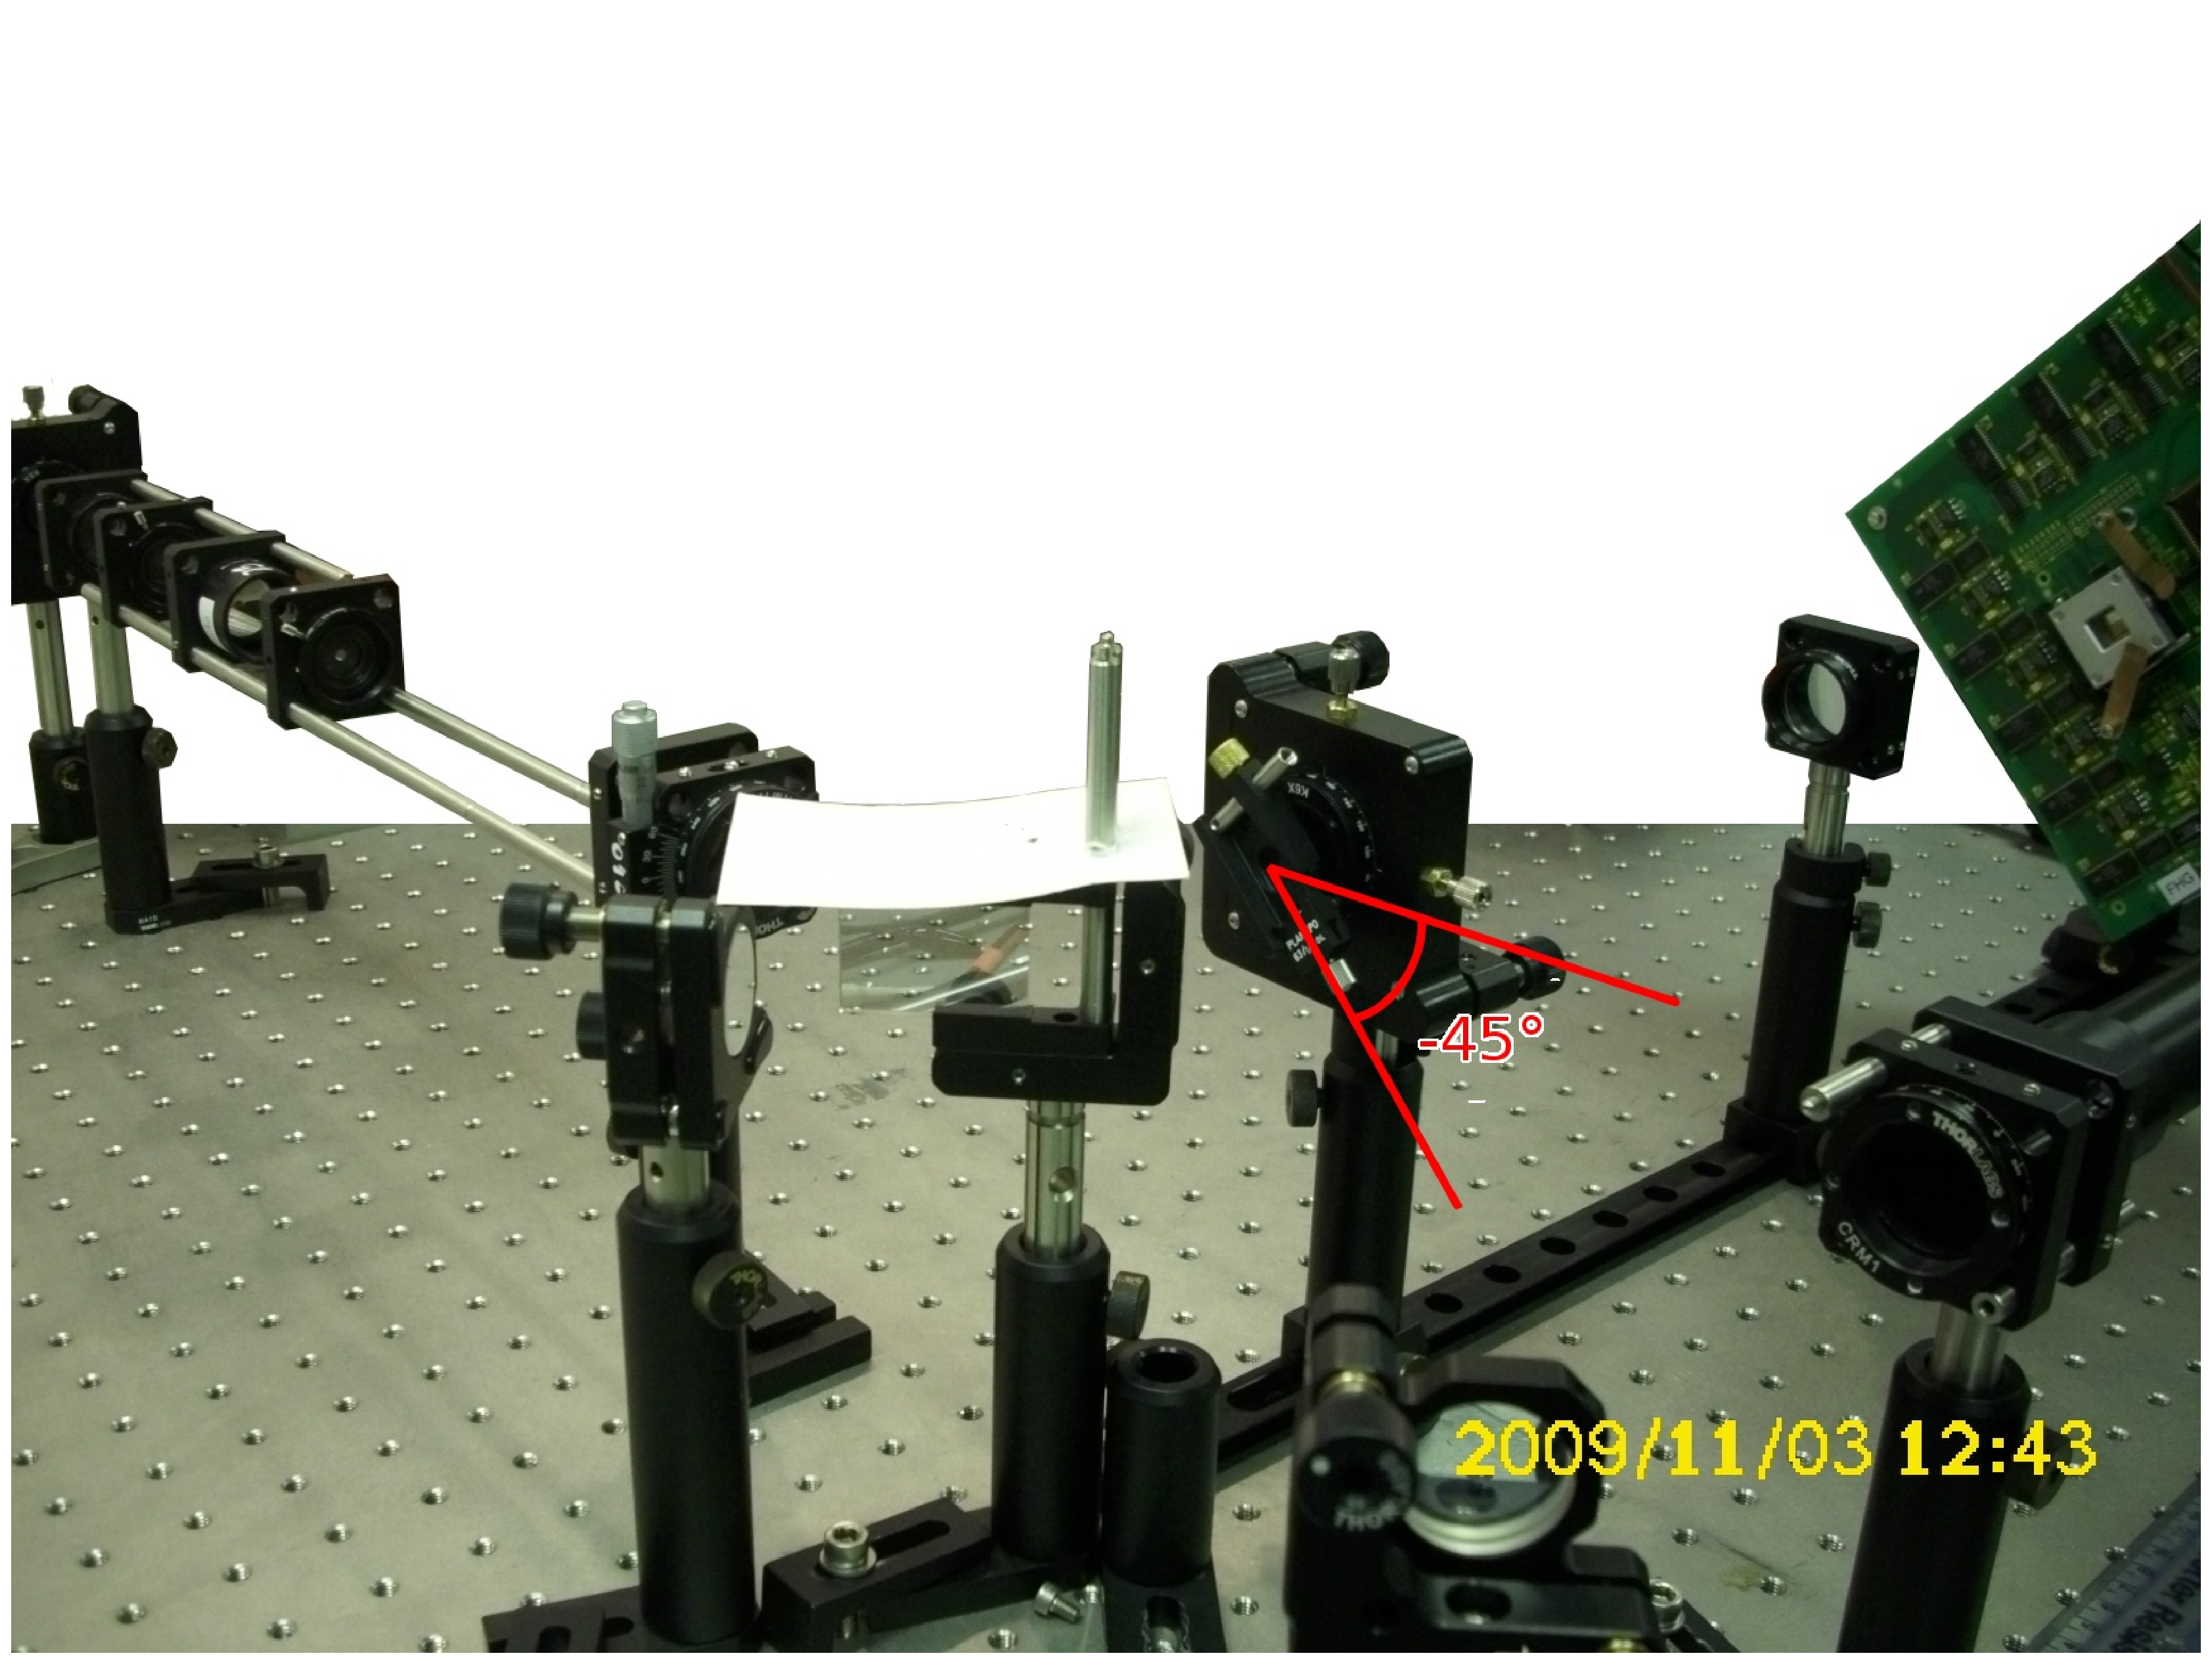
\includegraphics[width=9cm]{../app_dic/img/dsci1331}

  \caption{ Photo of the setup on the bench. Background has been
    removed for clarity. Here the Nomarski prism is oriented in
    $-45^\circ$ direction. Note that the MMA is rotated as well. The
    white paper card on top of the wire grid polariser protects it from
    dust.  This setup additionally includes two cleanup polarisers
    that are not shown in the schematic in \figref{fig:dic_mma}.}
  \label{fig:dic_photo}
\end{figure}

The illumination was improved by including an integrating rod which is
\unit[10]{cm} long. This gives a uniform light distribution on the
MMA.  The different incoherent LED light sources of our Cool-LED system
can be easily switched. However, the MMA is expected to give best
contrast for the LED with the shortest wavelength, which is
\unit[480]{nm}. Therefore all images in measurements in this report
were done with this LED.

The optical path for the illumination contains two apertures to
confine the field and to control the illumination angles (spatial
coherence).  We use a wire grid polariser (Moxtek, UT, US) as
polarising beam splitter.

The position of the focal plane of the Nomarski prisms was estimated
by measuring the distance between the Prism and the back focal plane
of the matching micro objectives (the result is generally
$\unit[2-3]{cm}$). The following procedure can be used to find the
correct focus of the Nomarski prism. For an unfocused prism one sees a
dark band that is transversally shifted when the bias of the prism
(its transversal position) is adjusted. The dark band gets wider when
the Nomarski prism is moved towards the focus. For the optimal setting
(and a planar object) the full field of view on the camera is dark.

We selected the prism with the biggest split angle
($\theta=\unit[0.078]{mrad}$, see section \ref{sec:prism} for the
measurement; matching a $63\times, 1.4$ oil immersion objective) in
order to keep the distances small and minimise beam distortion due to
air fluctuations. Later it turned out that the limiting factor is
actually the size of the prism. For a good DIC effect at least three
orders of the MMA diffraction pattern have to pass through the
prism. To ensure this two identical DIC prisms were used sequentially.

The objective lens and the MMA are positioned on a rail to simplify
focussing. The lens positions were pairwise adjusted by sending a
plane wave of a green laser through each ``telescope'' and checking
the outgoing wave with a shear plate. The distance of tube lens and
camera was set to the focal length by reflecting a parallel beam into
the tube lens and minimising the size of the spot on the camera.

\section{Model to describe the polarisation behaviour of the device}
\begin{figure}[htb]
  \centering
  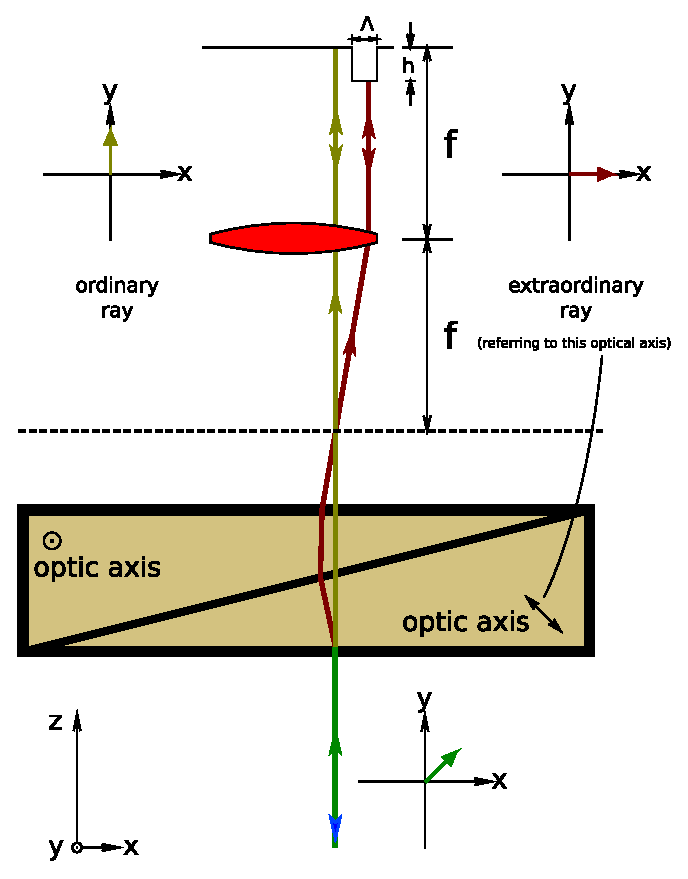
\includegraphics[width=6cm]{../app_dic/img/dic_prism}

  \caption{ Ray paths at the significant part of the setup: Linearly
    polarised light is split by the prism into two rays with slightly
    diverging angle. They hit the MMA at slightly different
    positions. The light returning through the Nomarski prism has
    different polarisation states depending on the difference $h$ of
    the mirrors at those two beam positions.  }
  \label{fig:prism}
%http://www.microscopy.fsu.edu/primer/java/polarizedlight/crystalwavefronts/index.html
\end{figure}
Here we consider the polarisation behaviour of light in our setup.
First we consider a simplified arrangement of one piston micro mirror
with width $\Lambda$ on a plane mirror (see \figref{fig:prism} for a
diagram).  Let $k=2\pi/\lambda_0$ with vacuum wavelength
$\lambda_0$. We then can write the influence of a retarder (the height
difference $h$ of the small piston mirror) on a polarised wave in
Jones calculus as (\cite{1996Goodman} p. 418):
\begin{align}
L_r(\Delta)=\begin{pmatrix}1&0\\ 0&e^{-i\Delta}\end{pmatrix}
\end{align}
with a phase difference $\Delta=2kh$ (the factor 2 due to the
reflection).  The matrix for a polariser that passes the component of
the electrical field which is linearly polarised at an angle $\alpha$
to the x-axis is:
\begin{align}
L_p(\alpha)=\begin{pmatrix}\cos^2\alpha&\sin\alpha\cos\alpha\cr
  \sin\alpha\cos\alpha&\sin^2\alpha\end{pmatrix}.
\end{align}
In our setup the incoming light has a $45^\circ$ polarisation $\vect
U=(1,1)^T/\sqrt{2}$ after the first reflection on the PBS. The light
passes through the Nomarski prism and is reflected by the MMA. Here
depending on the mirror height a phase retardation is imposed on one
of the two beams. The reflected light is recombined in the Nomarski
prism and only the component that is polarised at $\alpha=-45^\circ$
passes through the PBS onto the camera: $\vect
U'=L_p(-45^\circ)L_r(\Delta)$. We are interested in the intensity
$I'=|\vect U'|^2=(1-\cos\Delta$)/2.  For a piston mirror of width
$\Lambda$ the intensity of the output pixel is:
\begin{align}
  I_p=\int_0^\Lambda I'(\Delta(x'))\textrm{d}x'=\frac{\Lambda}{2}(1-\cos \Delta).
\end{align}
\begin{figure}[ht]
  \centering
  \includegraphics[width=7cm]{../app_dic/img/tilt}
  \caption{
Two mirrors that tilt with different deflections $d_1$ and $d_2$ in
opposite directions. The pitch of the mirrors is $\Lambda$. Note that
angles are exaggerated in this diagram.}
  \label{fig:tilt}
\end{figure}
As the mirrors of the MMA tilt (and don't move like pistons) it is
necessary to integrate along the DIC shift direction $x'$ to get the
brightness of one pixel depending on the tilt of the two neighbouring
mirrors (this calculation is done for small mirror tilts, see
\figref{fig:tilt}):
\begin{align}
\label{eqn:it}
  I_t=\int_0^\Lambda I'(\Delta(x')) \textrm{d}x'=\frac{\Lambda}{2}(1-\sinc(k \Delta d)).
\end{align}
Here $\Delta d=d_1-d_2$ is the difference between the deflections
$d_1$ and $d_2$ of the two mirrors and $\Lambda$ is the mirror pitch
(see \figref{fig:tilt}). Note that the integral does an incoherent
summation across the mirror. This is in order, as in our experiment we
use a LED light source. Note that the DIC image of torsion mirrors is
in general not constant over the width $\Lambda$ of one
mirror. Neighbouring mirrors do not differ in their height along the
pivot. Therefore there will always be a dark stripe in the centre of
the mirrors. If this device should be employed in the spatio-angular
microscope then these unwanted ``gratings'' should be taken into
account as they will affect the illumination in the LCOS (which sits
in the Fourier plane of the DIC image). This artifact doesn't occur
with piston style mirrors.

The scale factor of $I_t$ is arbitrary. In order to get a more useful
result we compare the brightness of MMA mirrors $I_t$ to a theoretical
device consisting of pistons that can move the distance $d$ from the
equilibrium position:
\begin{align}
\label{eqn:eta}
  \eta(\Delta d)=\frac{I_t}{I_p}=\frac{1-\sinc(k\Delta d)}{1-\cos(2kd)}.
\end{align}
\begin{figure}[ht]
  \centering
  \includegraphics{../app_dic/img/plot/deflection}
  \caption{Deflection curve for our generation-0 MMA sample (data
    supplied by Fraunhofer IPMS) and corresponding fit of cubic polynomial
    $d=a\cdot x^3+b$ with $a=\unit[(0.01136\pm0.0001)]{nm\, V^{-3}}$
    and $b=\unit[(4.32\pm0.3)]{nm}$. The x-axis is the voltage
    $U_\textrm{CE}$ that is applied to one of the electrodes of the mirror
    and the y-axis shows the deflection $d$ of the mirror (distance
    from mirror edge to the equilibrium position). The maximum voltage
    that we apply to the mirrors in our experiments is
    \unit[22.5]{V}. Assuming the extrapolation with the fit function
    is correct up to this voltage this corresponds to a deflection of
    \unit[134]{nm}. Half the deflection is then obtained at
    \unit[17.7]{V}. }
  \label{fig:deflection}
\end{figure}
The data sent to the generation-0 MMA are integers $q$ from 0 to 255
that set the voltage of the counter electrode $U_\textrm{CE}$
\begin{align}
U_\textrm{CE}(q)=s_\textrm{img}\cdot \unit[30]{V} \cdot \frac{q}{255}.
\end{align}
The scale factor $s_\textrm{img}$ is \unit[0.75]{} in our experiments.
With the device the Fraunhofer~IPMS delivered a transfer function for
the MMA that describes the relation between the voltage and the
deflection (see \figref{fig:deflection}). Note that this measurement
was done on an ensemble of micro mirrors with slight manufacturing
differences. This might explain why the deflection doesn't start with
zero. Also the data stops at $U_\textrm{CE}=\unit[18]{V}$ so we have
to rely on extrapolation to get the deflections for high voltages. If
that extrapolation is in order, the maximum deflection is:
\begin{align}
\label{eqn:dmax}
d_\textrm{max}=\unit[0.01136]{\frac{nm}{V^3}}\cdot(0.75\cdot\unit[30]{V})^3+\unit[4.32]{nm}
=\unit[(134\pm2)]{nm}.
\end{align}
For a wavelength of \unit[480]{nm} one gets $\eta=0.21$. So pistons
instead of torsion mirrors achieve five times higher brightness.

We hope that the transfer function of the generation-2 MMA will start
with a negative deflection. Only that way it will be possible to
adjust the micro mirrors for perfect flatness. This is necessary in
order to achieve high contrast with the Schlieren optical approach. It
is less important for the DIC method.

For the DIC method a pixel will be dark when both mirrors are tilted
the same way ($\Delta d=0$) and it will be brightest for a difference
in deflection $\Delta d=\lambda/2$. So if the mirrors don't tilt
enough to form a blazed grating the DIC method isn't expected to
achieve higher contrast than the Schlieren method.

\begin{figure}[ht]
  \centering
  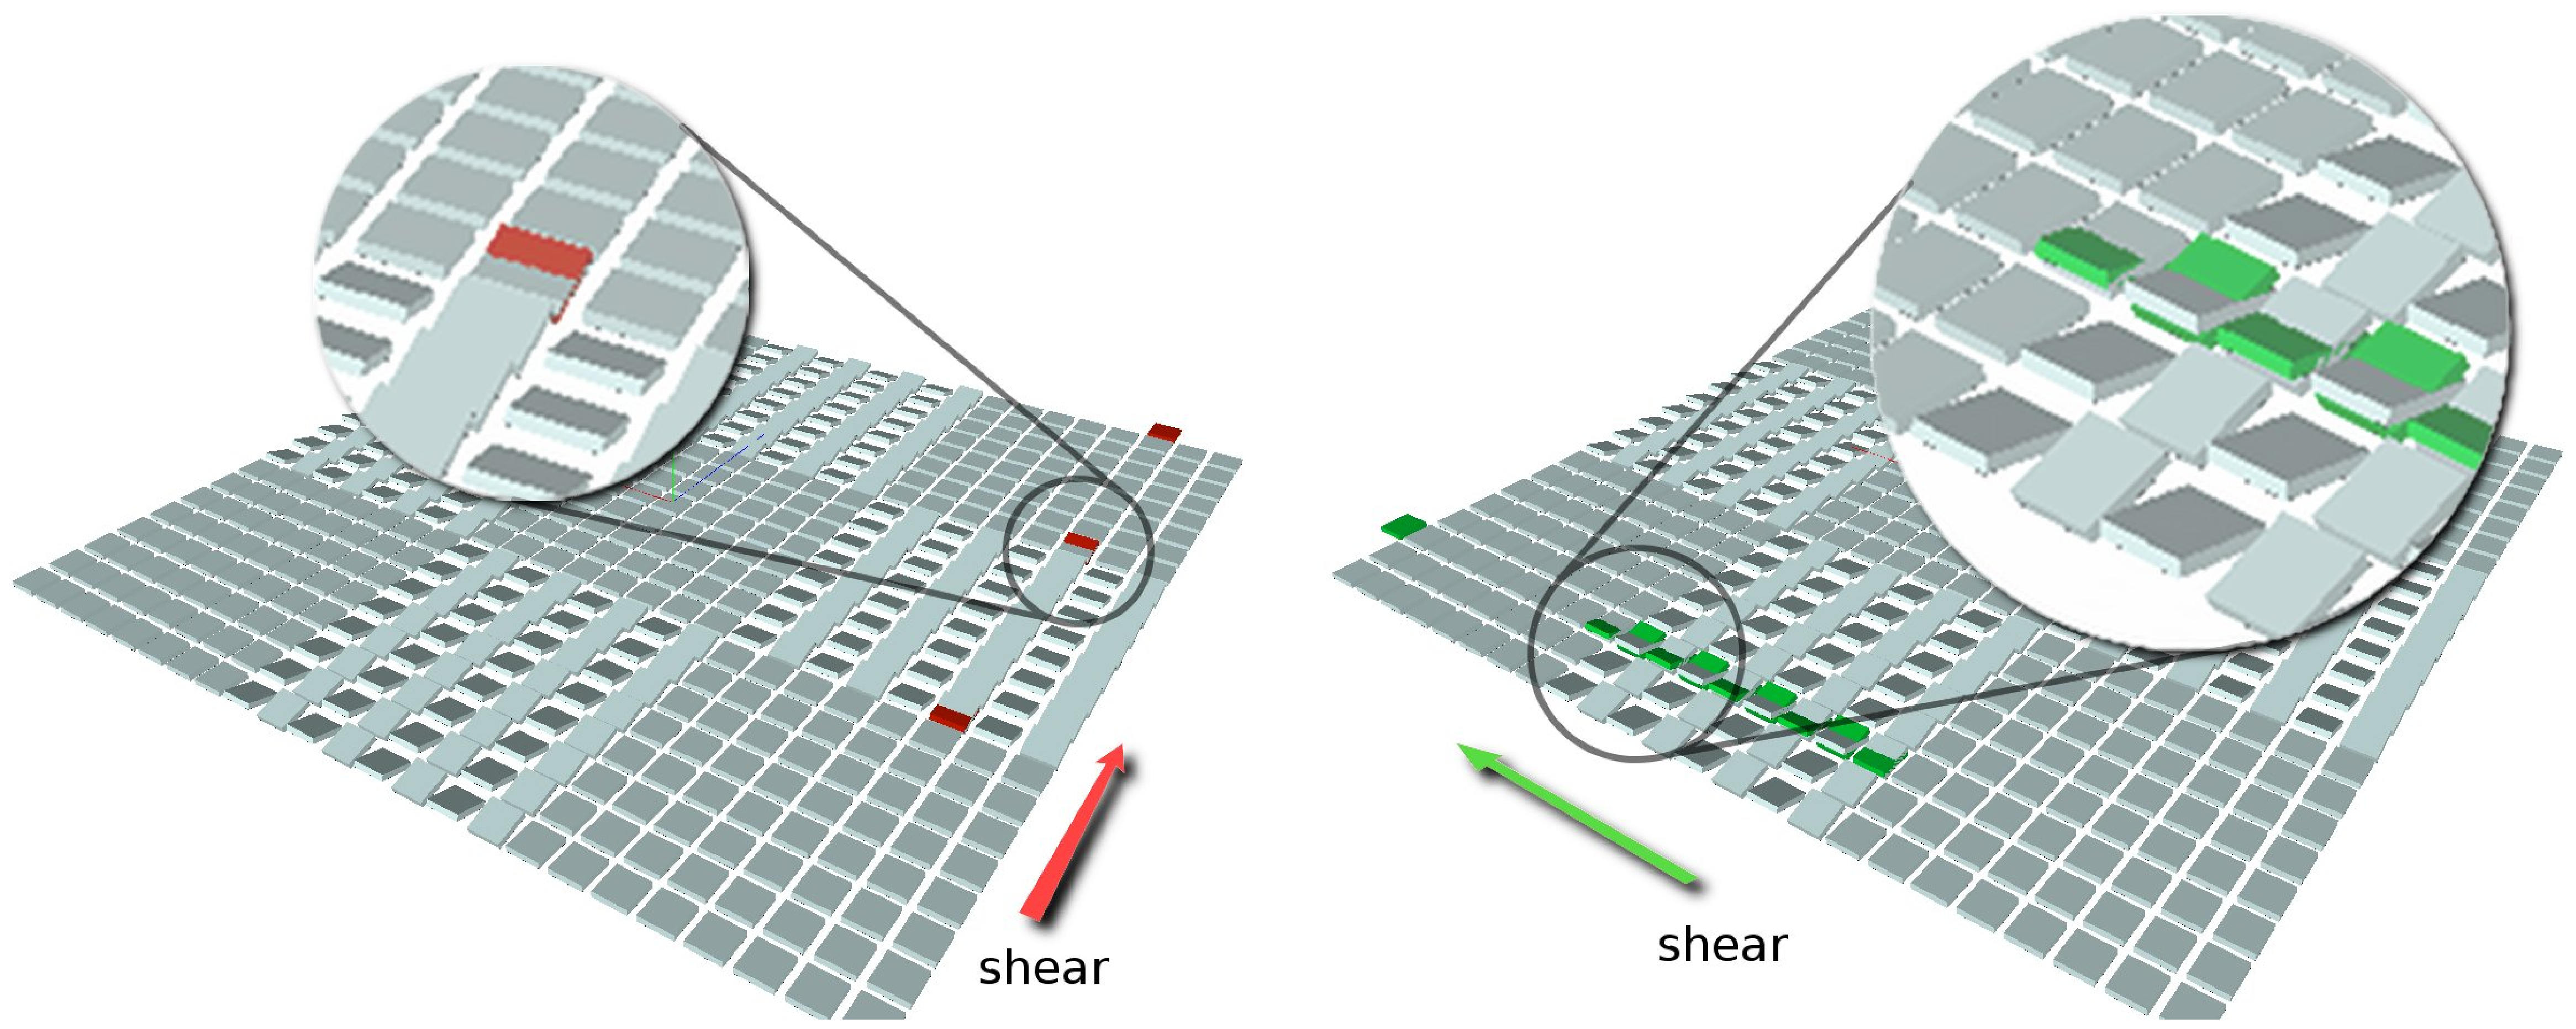
\includegraphics[width=\linewidth]{../app_dic/img/mma_sketch}

  \caption{ Diagrams showing how rows (Nomarski prism in $-45^\circ$
    angle, left) or columns (Nomarski prism in $+45^\circ$, right) of
    the MMA are overlayed by the DIC prism. The coloured parts depict
    the neighbouring mirror as it is overlayed by the DIC. These
    images only show a $24\times 24$ section of mirrors with a
    checkerboard of $16\times 16$ periodicity.}
  \label{fig:screen}
\end{figure}
\begin{figure}[htb]
  \centering
  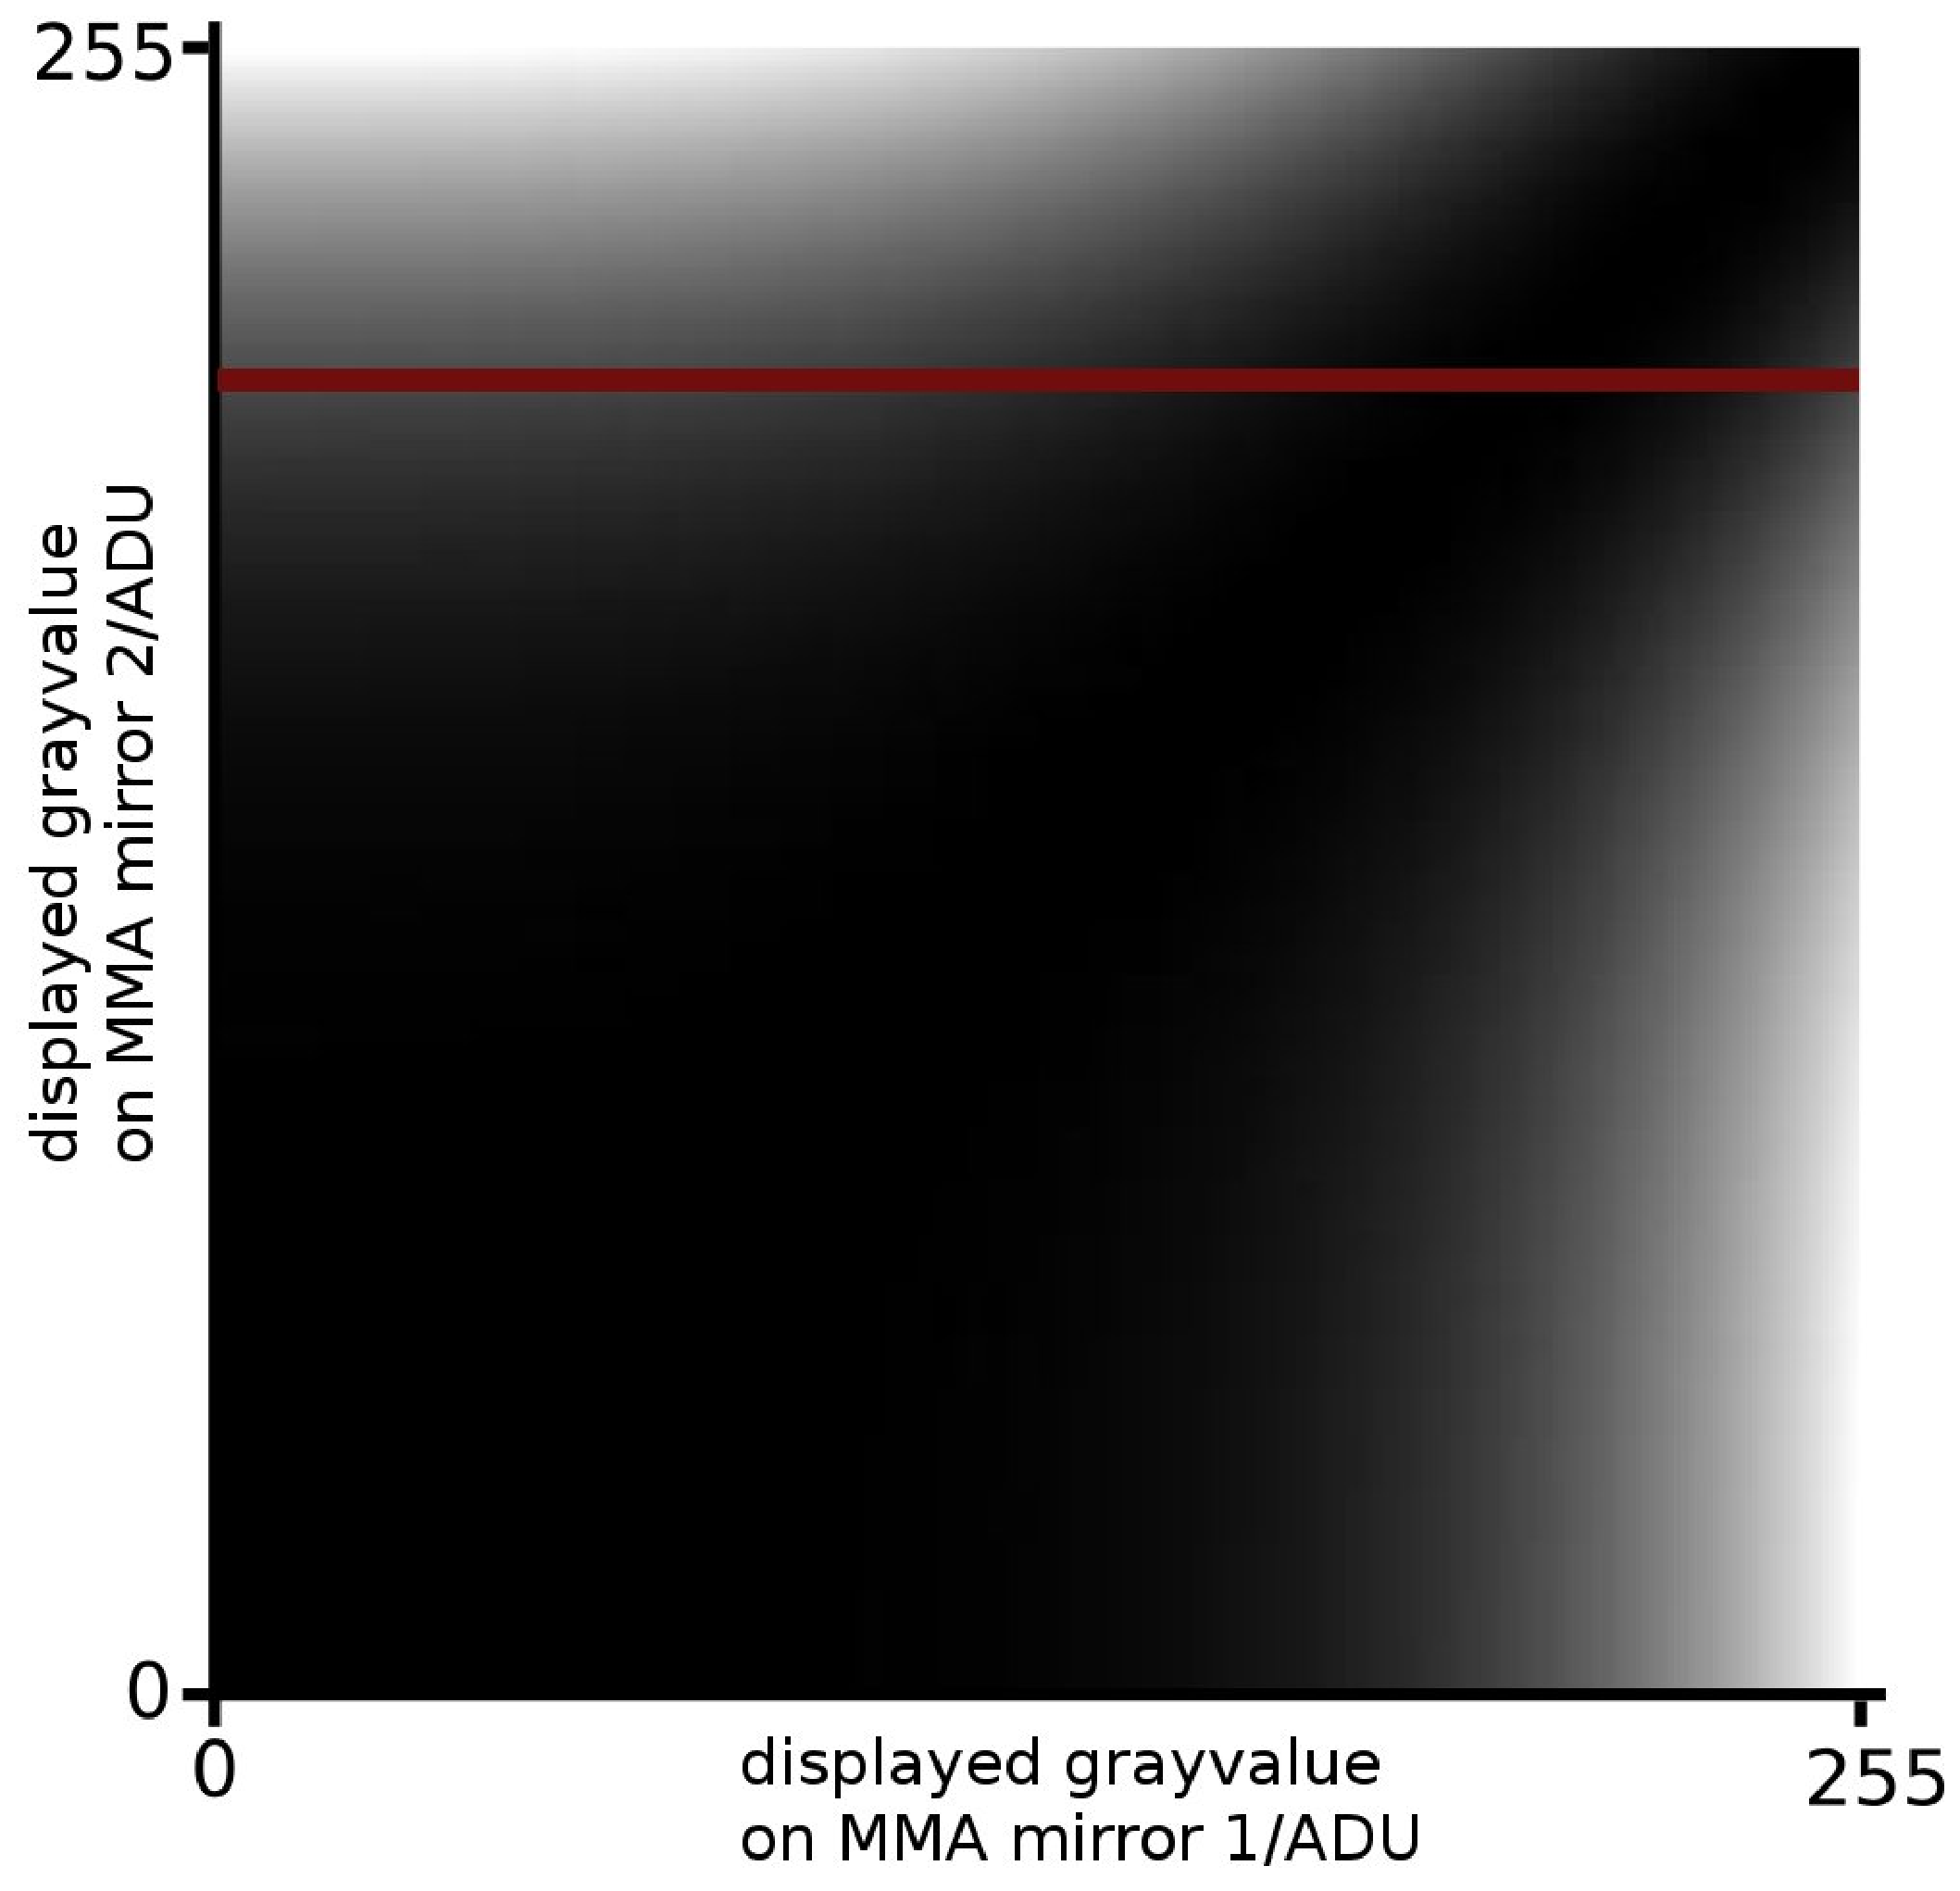
\includegraphics[height=6.5cm]{../app_dic/img/lut-plot}
  \includegraphics[height=6.5cm]{../app_dic/img/plot_lut/lut_graph}

  \caption{{\bf left:} Theoretical $\eta$ in dependence of the tilts
    of neighbouring mirrors. The arbitrary data units (ADU) are
    proportional to the voltage $U_\textrm{CE}$. An ADU of 255
    corresponds to a deflection of \unit[134]{nm}. Black corresponds
    to $\eta=0$ and white corresponds to $\eta=0.21$. {\bf right:} The
    graph shows the values along the red line in the matrix on the
    left, i.e. ``mirror 2'' is not tilted with gray value~200
    corresponding to a tilt voltage $U_\textrm{CE}=\unit[17.7]{V}$
    that deflects the mirror to half of the maximum possible
    deflection. The maximum brightness $\eta=0.064$ that can be
    obtained with this setting (when ``mirror 1'' is tilted to the
    maximum angle) is $30\%$ of the brightness for maximum tilt
    difference between two mirrors.}
  \label{fig:deflection2}
\end{figure}
Due to the bidirectional tilt of the mirrors along alternating rows
(see \figref{fig:screen}) the MMA allows two different DIC modes.
Either the mirrors are overlayed along rows (all mirrors tilt into the
same direction, see the left image in \figref{fig:screen}) or mirrors
are overlayed in column direction (neighbouring mirrors tilt to
opposite sides, see the right image in \figref{fig:screen}). The
latter mode we cannot employ to display arbitrary images.  Two
neighbouring flat mirrors will produce black and two opposite-tilt
mirrors will produce a maximum. However there is no way how these
mirror tilts can be adjusted such, that arbitrary images can be
generated.

When the DIC shear direction is the same as the mirror tilt direction
it is always possible to generate a black image pixel by setting two
immediate neighbours to the same tilt angle. In an analogues manner
one can create arbitrary gray values by tilting neighbouring mirrors
in slightly different directions. Equation \eqref{eqn:it} describes
the relation between tilts of the mirrors and the intensity of the
image pixel. The brightest value $\eta=21.4$ can be achieved when one
mirror is in the plane position and the neighbour is tilted to the
maximum possible deflection $d_\textrm{max}$ (equation
\eqref{eqn:dmax} shows its value for our generation-0 MMA).  However,
it is not possible to exploit the full dynamic range of the device
when arbitrary images are to be displayed (at least not with the
algorithm that we are going to describe).  Instead the maximum dynamic
range is from $\eta=0$ to $\eta=0.064$.

We now describe the algorithm that we use to calculate the mirror
tilts (actually the pixel values $q$) that will result in a given
intensity image after the DIC device. It uses our model of the DIC
device and the transfer function that maps voltages to mirror tilts.

Set a pixel on the border of the MMA to 0. We call this pixel ``mirror
2''. Then go one pixel in the direction of the DIC shift. We call this
pixel ``mirror 1''. Look in the target image what intensity should be
produced at this position after the DIC device. Search this intensity
in the look up table (\figref{fig:deflection2}) along the abscissa
(for gray value 0 of ``mirror 2'') and set the gray value of ``mirror
1'' to the corresponding gray value. Now rename ``mirror 1'' to
``mirror 2'' and go to the next pixel of the matrix. Repeat this
procedure for all pixels in this rows and do this algorithm for all
columns of the MMA.

Note that the overlay of the extraordinary and the ordinary image
might be rotated in the wrong direction when the prism orientation
isn't perfect. Also when the prism split angle doesn't match, the
images of two mirrors will not lie exactly on top of each other
leading to line like artifacts in the DIC image. However the two
images have by definition the same scale. So there are no beating
effects in the DIC image.

\section{Results}
In \figref{fig:screen5} you can see two typical images that can be
achieved with the DIC setup. On these images the mirrors of the MMA
tilt in $-45^\circ$ (to the bottom right) or in $+135^\circ$ (to the
top left).

The image that is displayed on the MMA for both pictures is a black
and white checkerboard with a periodicity of $16\times 16$ elements
(as in \figref{fig:screen}).  \figref{fig:screen5}~b) is the case that
is not usable for us. The DIC shift is along the $+45^\circ$ direction
and brings mirrors that tilt in different directions to interference.
The rectangles on the MMA where the mirrors are tilted appear bright
in this image. The regions where the mirrors are flat are dark in the
image. According to the right diagram in \figref{fig:screen} the
bright rectangles should have a darker border. Indeed this can be seen
in the image on the camera (look at the first row in the right height
profile in \figref{fig:screen5} (indicated by arrow)). Furthermore in
the middle of the pixels dark stripes can be seen. This is where the
torsion mirrors are fixed and have the same height.

\begin{figure}[p]
  \centering
  \includegraphics[height=5.9cm]{../app_dic/img/1219/auswert/1checker}
  \includegraphics[height=5.9cm]{../app_dic/img/1219/auswert/2checker}
  \includegraphics[width=7cm]{../app_dic/img/1219/auswert/1checker-section}
  \includegraphics[width=7cm]{../app_dic/img/1219/auswert/2checker-section}
  \includegraphics[width=7cm]{../app_dic/img/1219/auswert/1checker-height}
  \includegraphics[width=7cm]{../app_dic/img/1219/auswert/2checker-height-arrow}
  \caption{ DIC image for a prism setting of $-45^\circ$ (a) and
    $+45^\circ$ (b). Below both images a cross section in the
    direction of the DIC shift is shown (along the line marked with
    1)). The horizontal lines in those graphs show the values
    $I_\textrm{max}$ and $I_\textrm{min}$ for contrast estimation. The
    contrast ratios are \unit[0.62]{} for (a) and \unit[0.65]{} for
    (b). The rectangular region that is marked with 2) in the images
    is displayed as height maps. These images were taken with two
    identical sequential DIC prisms (for $63\times\,,1.4$), a
    \unit[100]{mm} objective lens and a \unit[300]{mm} tube lens.}
  \label{fig:screen5}
\end{figure}

In \figref{fig:screen5}~a) you can see the corresponding image with
the prism turned by $90^\circ$ relative to the right image. The
displayed image on the MMA is the same black and white
checkerboard. According to the left diagram in \figref{fig:screen} one
would expect white lines perpendicular to the shift direction. The
image on the camera has these features and again one can make out the
dark lines in the centres of the pixels.

The contrast ratio for this experiment is only \unit[0.6] and also the
contrast in \figref{fig:screen5}~b) isn't much higher. This is
probably because two identical DIC prisms were used in sequence to
achieve twice the split (see \figref{fig:double-prism}). Without this
disputable trick a \unit[200]{mm} lens has to be used to get the
necessary $\unit[16]{\mu m}$ DIC split but then the Fourier pattern is
too big for the size of our DIC prisms. So right now we are stuck with
two different suboptimal solutions to split the beam.

\begin{figure}[htb]
  \centering
  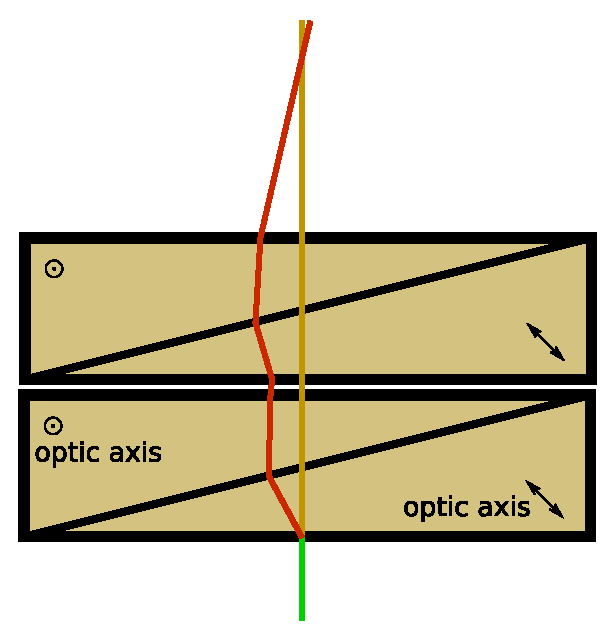
\includegraphics[width=5cm]{../app_dic/img/double-prism}
  \caption{Combination of two identical DIC prisms to increase the
    split. The prism in the experiments are for a $63\times,\,1.4$ oil
    immersion objective.}
  \label{fig:double-prism}
\end{figure}

Nonetheless we tried to produce gray value images.
\figref{fig:erika-overview} shows the gray value image that should be
displayed on the camera. The image that has to be displayed on the MMA
is shown in \figref{fig:erika-detail}~b) and
\figref{fig:erika-detail}~c) shows the result on the camera (for the
two DIC prism setup).

In section \ref{sec:size} some measurements for the setup with a
\unit[200]{mm} objective lens and only one prism are shown.

\begin{figure}[p]
  \centering
  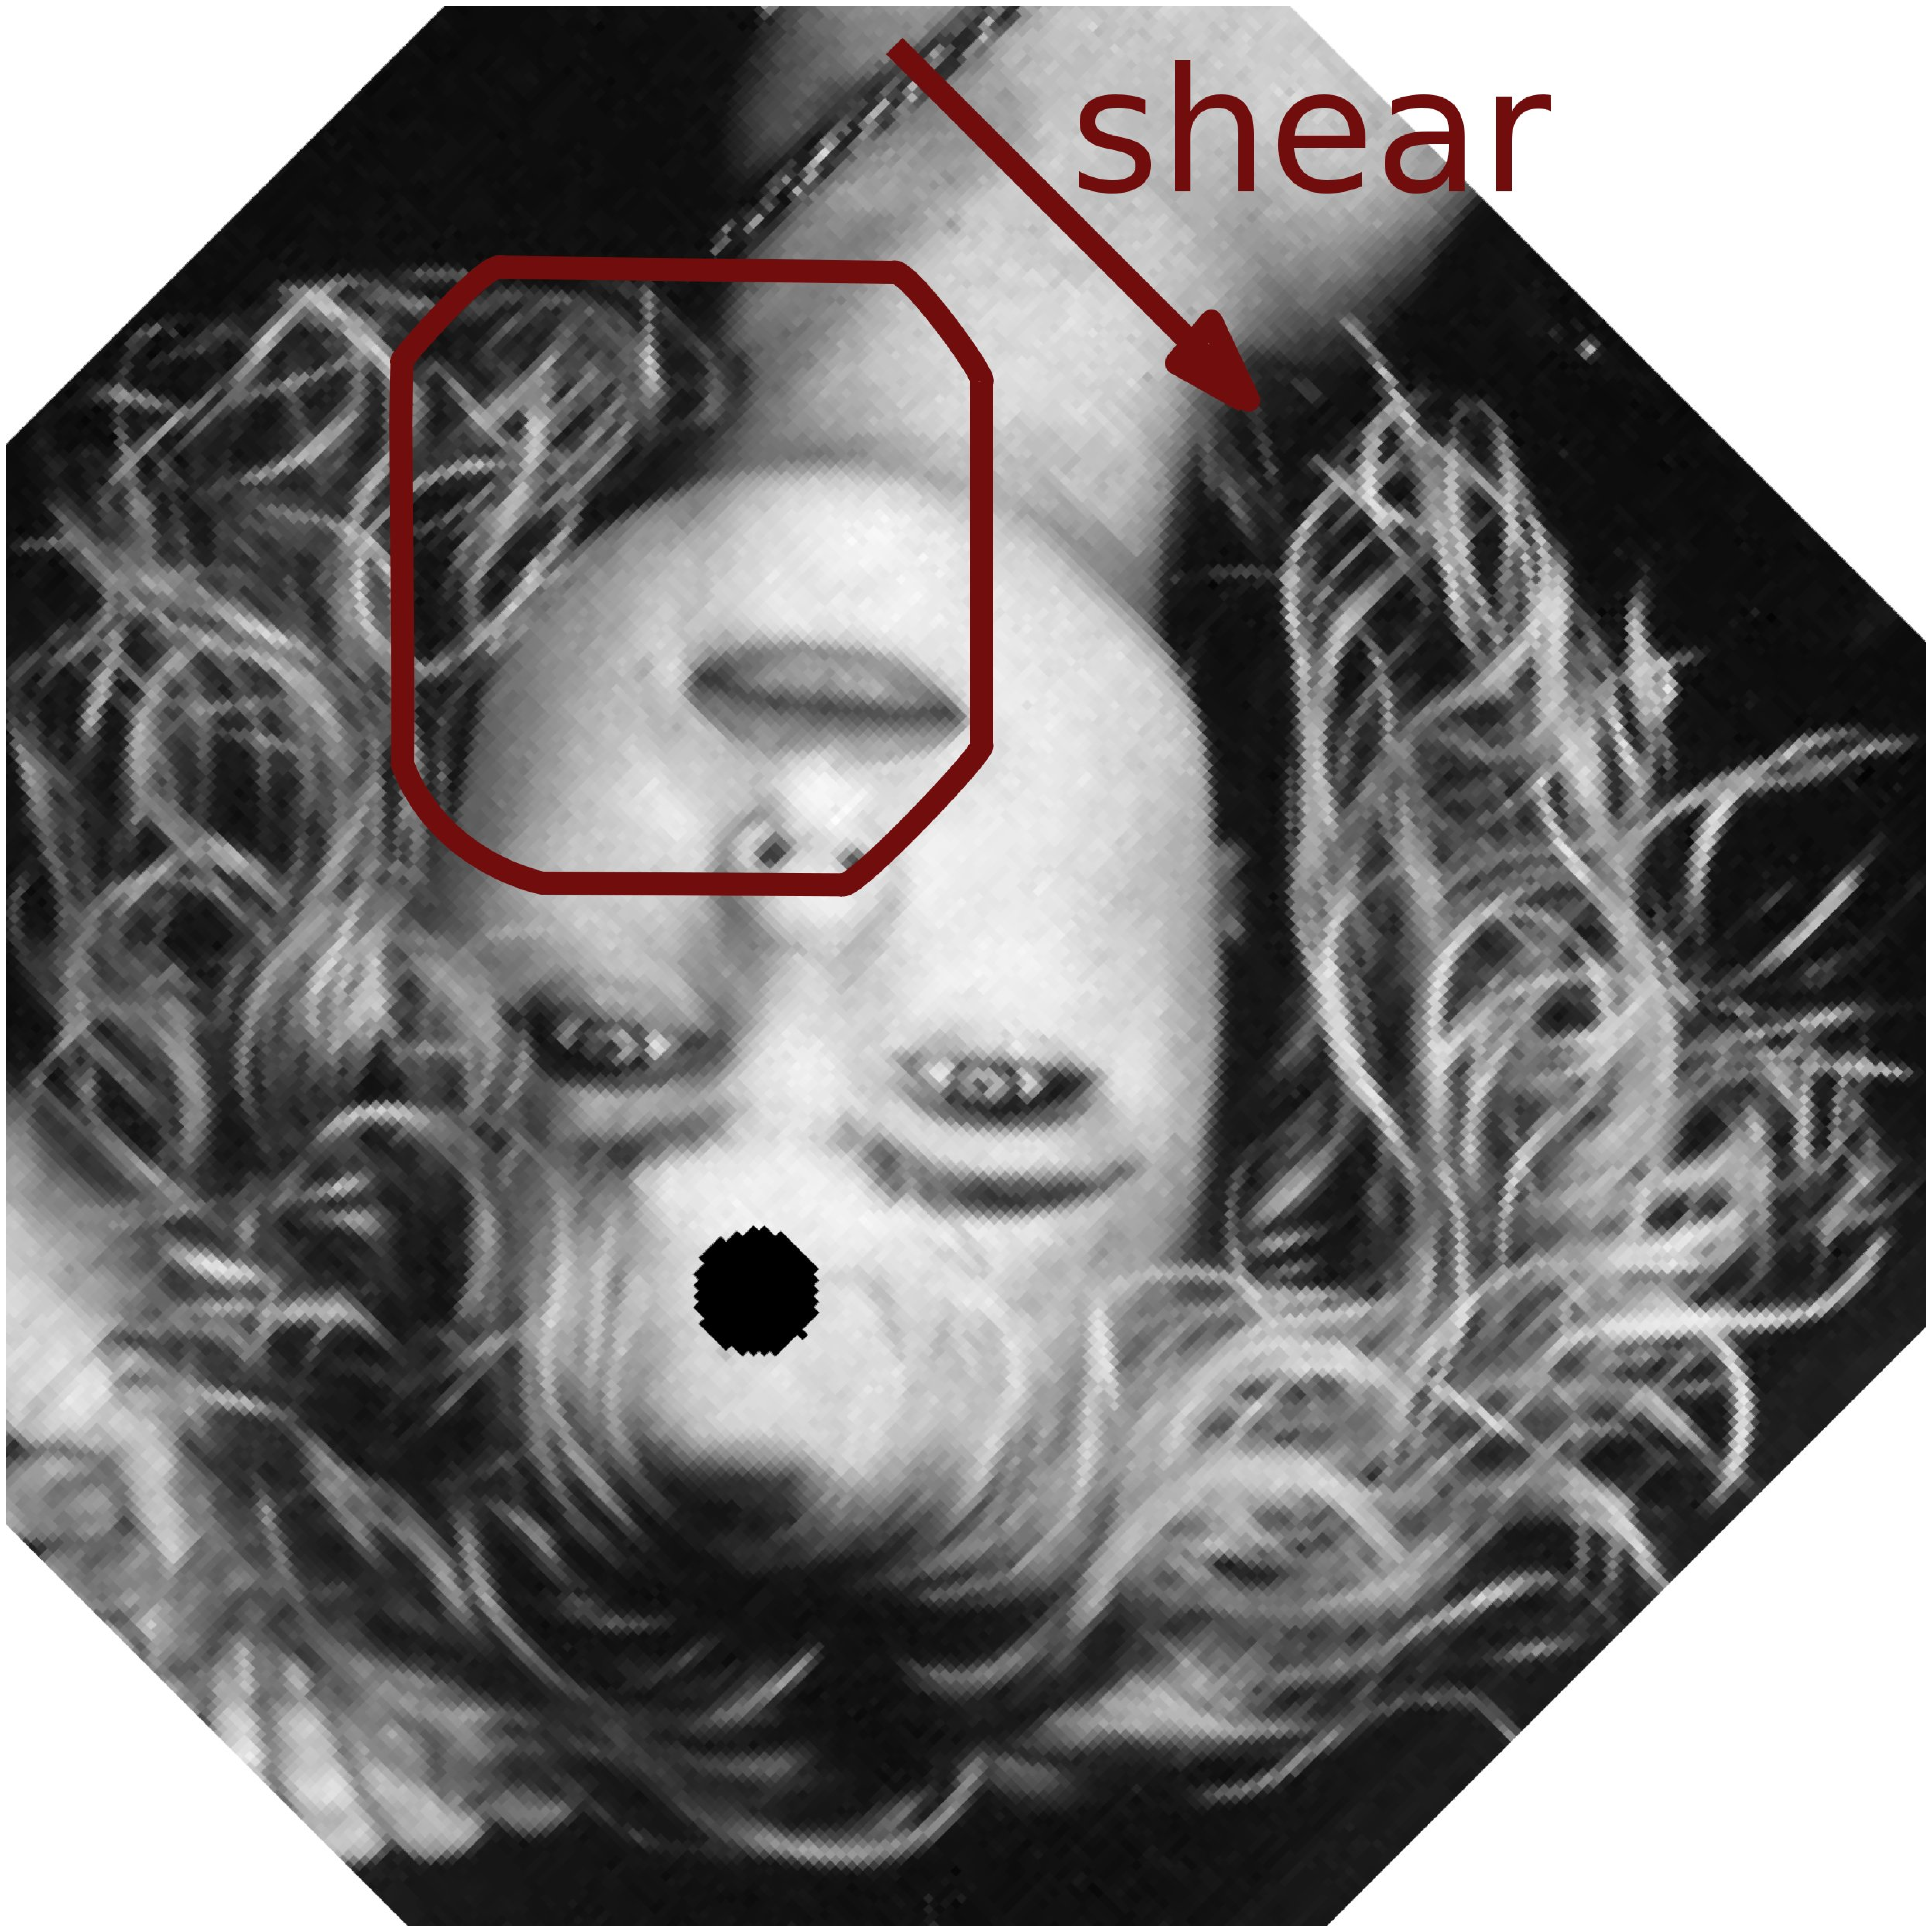
\includegraphics[width=7cm]{../app_dic/img/1219/auswert/erika-overview}
  \caption{The input image that should be displayed on the camera. The
    rectangular region is illuminated by the integrating rod and
    imaged on the CCD.}
  \label{fig:erika-overview}
\end{figure}

\begin{figure}[p]
  \centering
  \includegraphics[width=\linewidth]{../app_dic/img/1219/auswert/erika-detail}
  \caption{{\bf (a)} Closeup of the input image. {\bf (b)} The
    precomputed (with the look up table algorithm as listed in section
    \ref{sec:source}) image that is displayed on the MMA. The DIC
    shift will occur from the left top towards the right bottom. Note
    that regions that are white in the input image have a grating
    structure with high contrast. {\bf (c)} The resulting image on the
    camera.}
  \label{fig:erika-detail}
\end{figure}

\section{Discussion}
With the new setup we showed that the pure DIC method (without Fourier
filtering) allows to create an intensity image from a phase device.

The theoretical considerations lead to the conclusion that a piston
device possesses two significant advantages compared to the torsion
mirrors. The DIC prism has to be big enough so that at least three
orders of the diffraction pattern of the torsion mirrors can form an
image. Torsion mirrors always have a black line in the centre of the
pixel because here neighbouring mirrors have the same height. A piston
device therefore will achieve higher contrast with a smaller prism.

For optimal performance it is crucial to have the MMA exactly in
focus. Currently it is very hard to focus the MMA as it is fixed to a
large printed circuit board with a heavy cable. After each focus
change the angle of the board generally has to be readjusted so that
the zero order goes back through the Nomarski prism. With the next
generation MMA this problem should be solved as the device is
connected to the circuit board by a flexible cable.

As an interesting application of the DIC method (other than improving
the contrast) it might be possible to determine characteristic
deflection curves for all mirrors of a device individually. One
approach would be to set all the mirrors parallel to the device
surface with a $+45^\circ$ DIC setting and then check for blackness
with a $-45^\circ$ setting and different voltages applied to
neighbouring mirrors. With a device that is calibrated in such a way
even better contrast will be possible, as mirror tilts can be adjusted
to be exactly equal (with an uncalibrated device there is some spread
due to manufacturing differences). Right now no programmable update of
images is possible so no such iterative calibration algorithm has been
implemented.

\begin{figure}[p]
  \centering
  \includegraphics[width=1.5cm]{../app_dic/img/trickwedge}
  \caption{DIC ``prism'' with adjustable wedge (based on Figure 3
    in the patent \cite{1960Nomarski}).}
  \label{fig:trickwedge}
\end{figure}

To further improve the setup it will be necessary to obtain a matching
prism.  Nomarski's patent \cite{1960Nomarski} already describes a
prism with an adjustable wedge angle. It consists of two quartz
plano-concave cylinder lenses (see \figref{fig:trickwedge}). When the
two lenses are shifted transversally, one obtains in effect a wedge
with adjustable angle.

Another option would be to use a birefringent plane with the a skew
optic axis. The ordinary and extraordinary beam that leave this plate
will be parallel. One could put this device in an image
plane. % Rainers Vorschlag, mit der image plane

Other alternatives to tune the split angle include changing the
wavelength of the light, heating the wedge material or applying an
electric field on the crystal.

\section{Acknowledgements}
We thank Kai Wicker for helpful discussions on the polarisation
issues.

\section{Nomarski prism}
\subsection{Procedure to measure the split angle}
\label{sec:prism}
The Nomarski prism consists of two quartz wedges. Its function is
based on the birefringence of the crystal. The prism splits a
$45^\circ$ linearly polarised wavefront into two wavefronts with
slightly diverging angles.
\begin{figure}[htb]
  \centering
  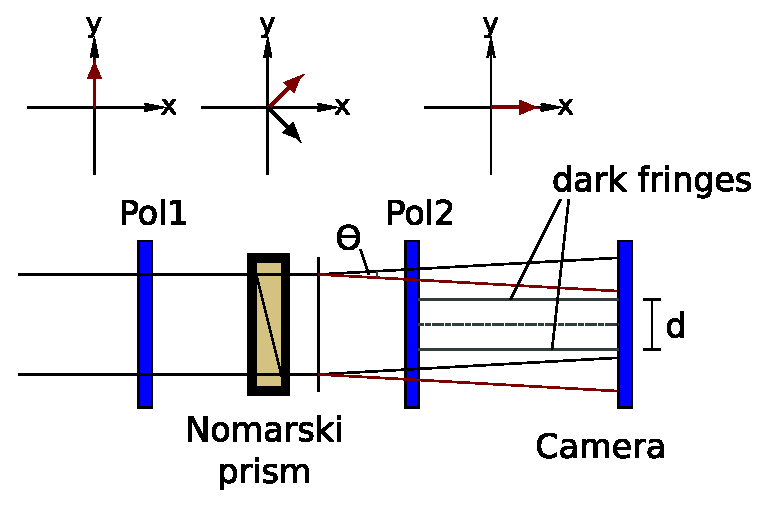
\includegraphics[width=8cm]{../app_dic/img/nomarski_split}
  \caption{Setup to measure the split angle $\theta$ of a Nomarski
    prism by interference of the two beams. The polarisers Pol1 and
    Pol2 are crossed and in a $45^\circ$ angle relative to the shift
    axis of the prism.}
  \label{fig:nomarski_split}
\end{figure}
The split is so small that its direct measurement (illuminating the
prism with a parallel beam and putting the camera into the back focal
plane of a lens with a long focal length) is hard.  So instead we put
the prism between crossed polarisers, illuminate it with a parallel
beam and measure a fringe system on the camera (see
\figref{fig:nomarski_split}
for a diagram and
\figref{fig:nomarski_split_exp}
for the data).

The electrical field $U$ after the second polariser is:
\begin{align}
  U&=e^{i\vect k_1\vect r}+e^{i\vect k_2\vect r},\\
  \abs{\vect k}&=\frac{2\pi}{\lambda},\\
  \vect k_1&=\abs{\vect k}(0, \hspace{1em}\sin(\theta/2), \cos(\theta/2))^T,\\
  \vect k_2&=\abs{\vect k}(0, -\sin(\theta/2), \cos(\theta/2))^T.
\end{align}
The camera measures the intensity $I$:
\begin{align}
  I=\abs{U}^2=4\cos^2(\abs{\vect k}y\sin(\theta/2)).
\end{align}
Therefore the dark bands have a distance $d$ (for small split angles
$\theta$):
\begin{align}
  d=\frac{\lambda}{2\sin{\theta/2}}\approx \frac{\lambda}{\theta}.
\end{align}
\begin{figure}[htb]
  \centering
  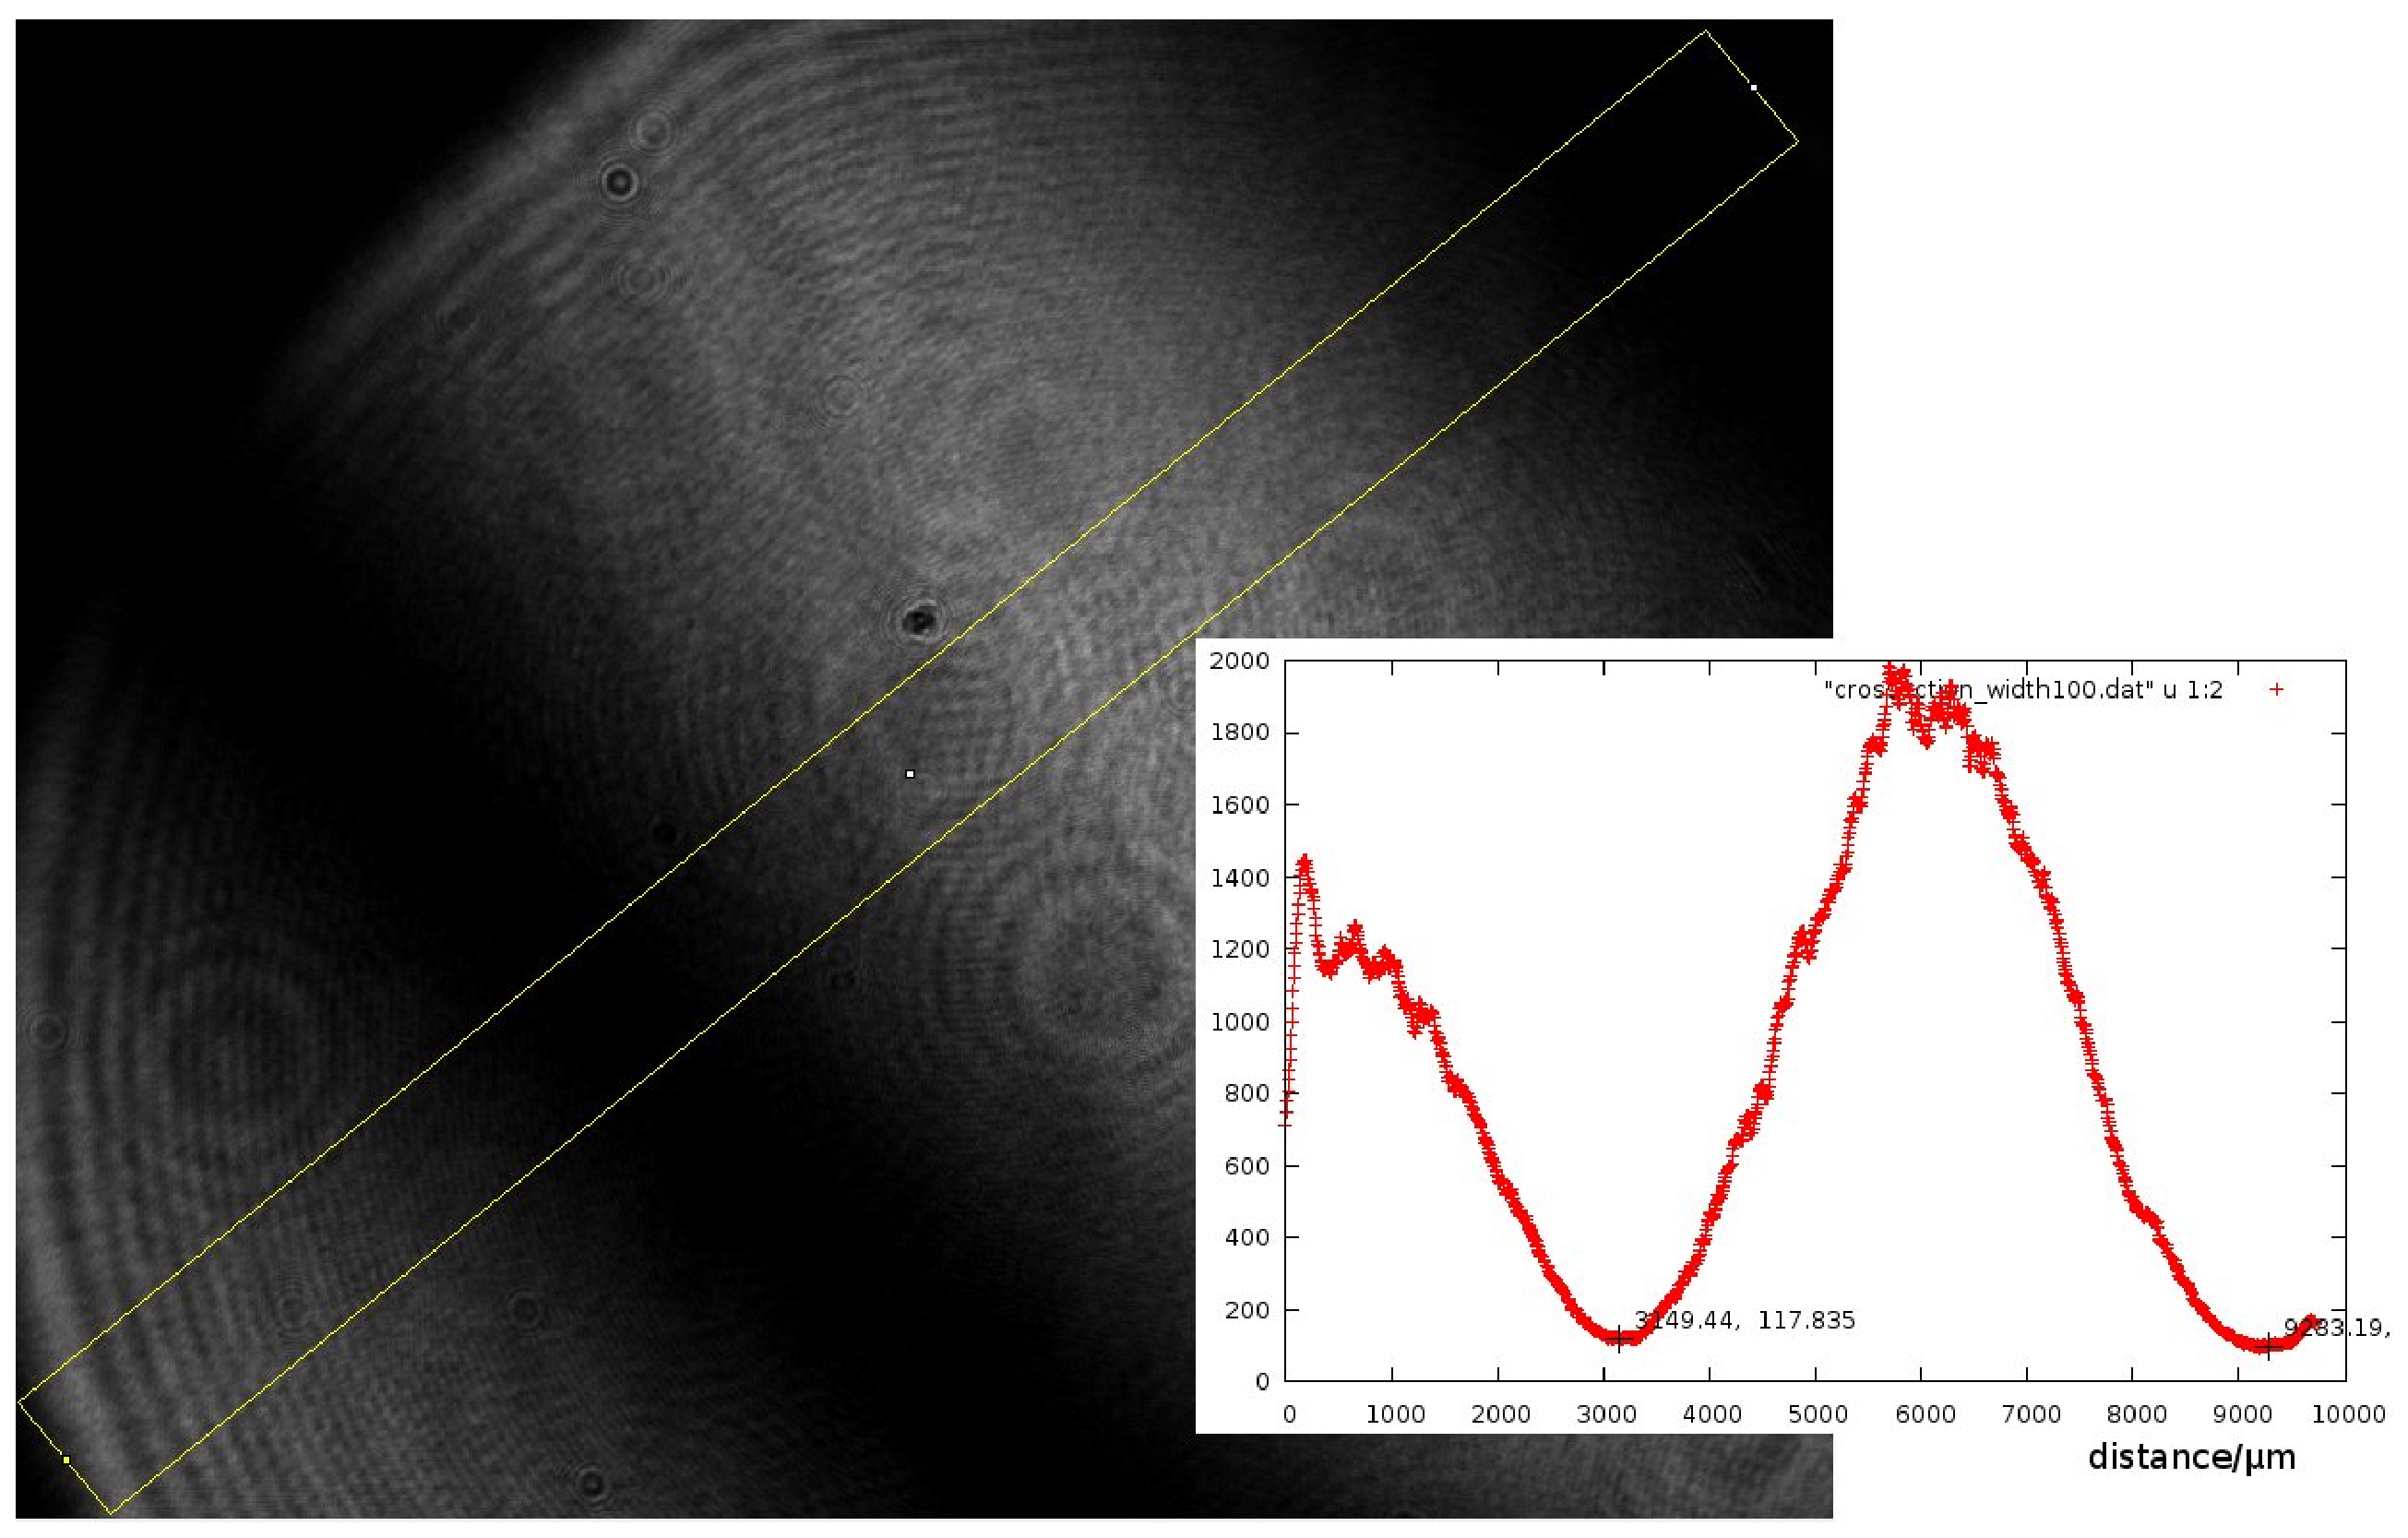
\includegraphics[width=10cm]{../app_dic/img/nomarski_split_exp}
  \caption{Camera image for the prism with the biggest split. The
    distance between the two dark fringes is
    $d=\unit[(6.06\pm0.08)]{mm}$. The light source is a laser with
    \unit[473]{nm} wavelength. The values over the width of the bar
    were integrated to reduce the influence of the disturbing fringes
    on the cross section.}
  \label{fig:nomarski_split_exp}
\end{figure}
Our prism has a split angle $\theta=\unit[0.078]{mrad}$.
For a lens with a focal distance $f=\unit[200]{mm}$ this corresponds to a
Nomarski split $\Delta x$:
\begin{align}
  \Delta x=2f\tan(\theta/2)\approx f\theta=\unit[(15.6\pm0.2)]{\mu m}.
\end{align}
This is close to the pixel pitch of $\unit[16]{\mu m}$ of the MMA.



\subsection{Construction of refraction at a birefringent surface}
\label{sec:raytrace}
For our setup it is not important that the beams cross outside of the
prism. This is just necessary when the back focal plane is inside of a
micro objective (behind lenses). One could as well use a Wollaston
prism (in these prisms the optic axes are in the transversal plane)
where the crossing would occur between the to wedges.  Or -- even
simpler -- just a birefringent wedge that is complemented to a
parallel plate with a glass wedge \cite{1960Nomarski}.

For a better understanding of what is going on in these crystals we
explain here how to construct the refracted rays on a birefringent
surface \cite{1991Saleh}. For the diagrams we assume a ray entering
from air and a crystal with a high birefringence. The effects in
quartz will be much less pronounced than in our diagrams
($n_e=1.54811$ and $n_o=1.53917$). Let us consider an incoming ray
with wave vector $\vect k_{in}$ and a polarisation perpendicular to the
optic axis (\figref{fig:refraction_pub_ord}~a)). In order to
construct the refracted ordinary wave vector $\vect k_o$ one draws a half
circle of radius $2\pi/\lambda$ below the surface (in air) and another
half circle with radius $n_o2\pi/\lambda$ in above the surface (in the
crystal). The normal component of the wave vector is conserved. Mirror
$\vect k_{in}$ at the surface normal and extend the normal through tip of
the mirrored wave vector and determine the intersection with the big
circle in the crystal. This is the wave vector $\vect k_o$ of the ordinary
ray and also the direction of the pointing vector $\vect S_o$.

For the other polarisation the construction of the extraordinary wave
vector $\vect k_e$ (see \figref{fig:refraction_pub_ord}~b)) is similar
but instead of intersecting a circle there is an angle dependent
refractive index (indicatrix ellipse) in the crystal.  Furthermore the
direction of energy transport $\vect S_e$ for the extraordinary ray isn't
collinear with the wave vector $\vect k_e$. To determine the direction of
$\vect S_e$ one has to construct the normal on the ellipse at the tip of
$\vect k_e$. This normal is the bisector angle between the foci and the
point on the periphery. \figref{fig:refraction_pub_ord}~d) finally
displays the refracted ray directions.
\begin{figure}[htb]
  \centering
  \includegraphics[width=\linewidth]{../app_dic/img/refraction_pub_ord}
  \caption{Construction of refraction at the surface of an uniaxial
    birefringent crystal for arbitrary angles of the optic axis.}
  \label{fig:refraction_pub_ord}
\end{figure}

\begin{figure}[htb]
  \centering
  \includegraphics{../app_dic/img/dic-raytrace}
  \caption{Ray trace through a Nomarski prism as shown in
    \figref{fig:prism}. The angle of the wedge and the birefringence
    is exaggerated and much bigger than in a real Quartz Nomarski
    prism. The computer program to create this construction is listed
    in section \ref{sec:source-raytrace}.}
  \label{fig:dic-raytrace}
\end{figure}

\subsection{Effects of limited crystal size on DIC image}
\label{sec:size}
The split angle of the DIC prism defines the focal length of the
objective lens that needs to be used because the shift on the MMA must
be at least $\unit[16]{\mu m}$. Our prism with the biggest split needs
a \unit[200]{mm} lens. However the free aperture of the prism is only
\unit[10]{mm}. Therefore it is problematic to capture three orders in
the image on the camera. These orders are needed to get an object like
image so that the DIC method does actually work.

For \figref{fig:erikas} one DIC prism was used with a \unit[200]{mm}
objective lens. It is not possible to get the two outside orders with
their complete surrounding information through the prism. The relative
size of the diffraction pattern on the DIC prism aperture is shown on
top of the images in \figref{fig:erikas}. Note that the angular extend
of the illumination in this case was approximately the same one would
use with the Schlieren optical system.

The main advantage of the DIC method -- and here we didn't make use of
this -- is that the angular extend of the illumination can be
significantly increased. Then the red dots grow bigger and may
overlap. However all the red dots should pass through the DIC prism.

In this experiment most of the dots were cut off. This leads to some
artifacts that are more pronounced when the aperture of the prism is
artificially shrunken (with a circular aperture).

The experiment showed that the artifacts originate from phase
continuities in the grating that is shown on the MMA (see
\figref{fig:erika-streak-overview}) for a closeup of one such region.
For this particular image it was possible to reduce the number of
phase discontinuities on the face by starting the look up table
algorithm on a central column and then computing to the left and the
right.

However even with this trick there are still some phase jumps after
strong gray value discontinuities in the input image (see the red
arrows in \figref{fig:erika-streak-overview}). One might try to
improve the algorithm to get rid of those as well but it is certainly
not good to cut of the orders. So the only real solution is to make
the prism bigger.

\begin{figure}[htb]
  \centering
  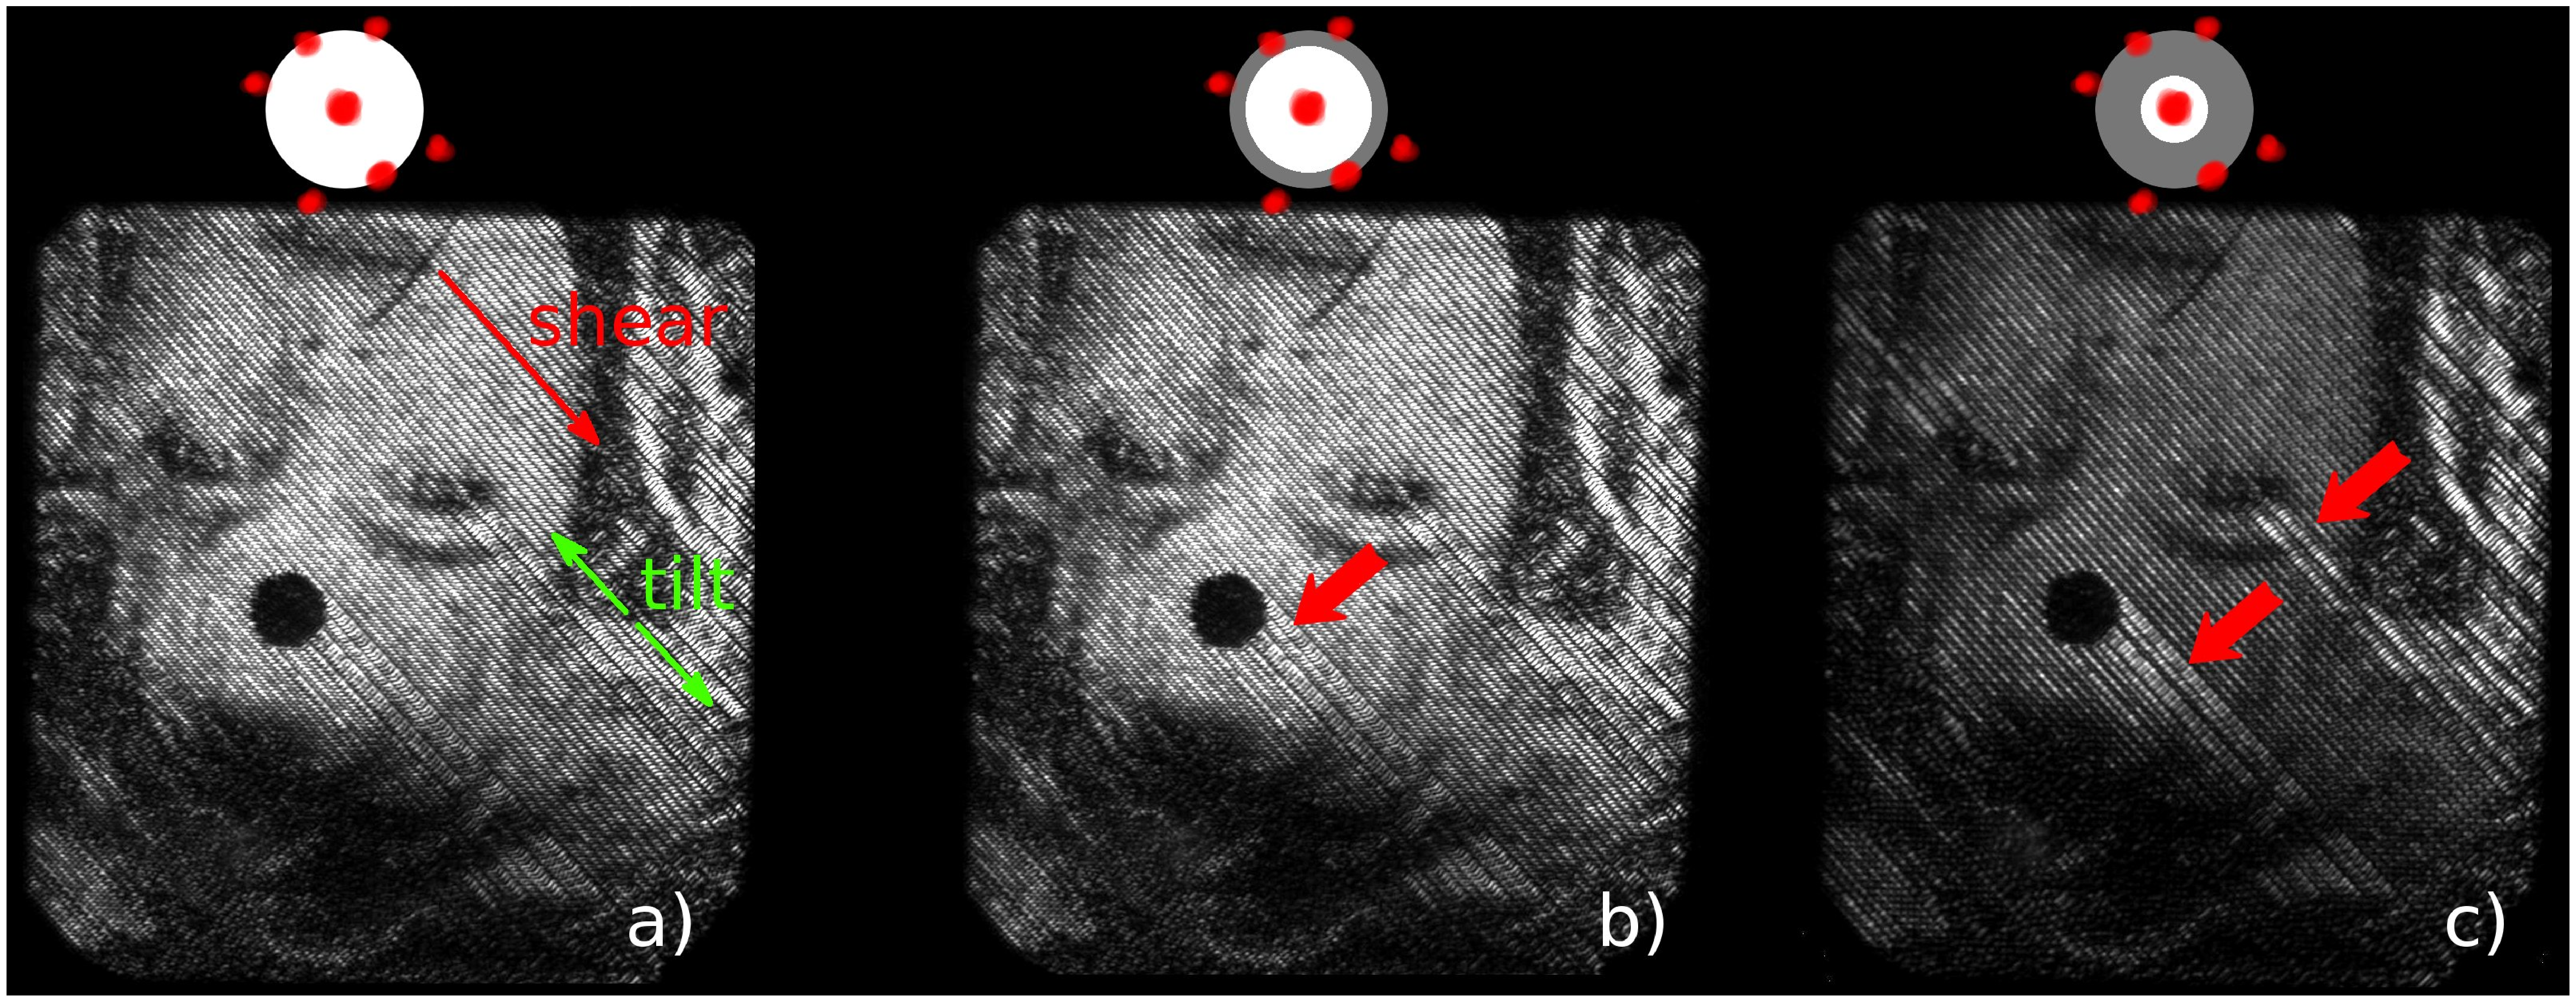
\includegraphics[width=\linewidth]{../app_dic/img/streaks2}
  \caption{These three images show artifacts in gray level images that
    arise when less than three orders contribute to the image. The
    diagram in the top shows the aperture diameter in relation to the
    Fourier pattern of the MMA device. Phase changes in the displayed
    MMA image (see \figref{fig:erika-streak-overview}) result in
    banding artifacts (see red arrows) for decreasing aperture
    diameter. These images were taken with one DIC prism (for
    $63\times\,,1.4$ micro objective) a \unit[200]{mm} objective lens
    and a \unit[500]{mm} tube lens.}
  \label{fig:erikas}
\end{figure}

\begin{figure}[p]
  \centering
  \includegraphics[width=\linewidth]{../app_dic/img/1219/auswert/erika-streak-overview}
  \caption{This image is displayed on the MMA in order to create a
    gray value DIC image. The shear direction is from top left to
    bottom right. When neighbouring image values are black and white
    the resulting pixel on the camera will be bright. If the image
    values don't change (look e.g.\ at the inside of the black circle)
    the pixel will be dark on the camera. When a dark gray value is to
    be generated there are many gray value pairs that result in the
    same intensity after the DIC device. However, if not all Fourier
    orders contribute to the camera image this is not true. Especially
    phase steps (see red arrows) produce banding artifacts. Note that
    this image generates a gray value image without artifacts when the
    two DIC prisms with a \unit[100]{mm} lens are used.}
  \label{fig:erika-streak-overview}
\end{figure}
\section{Source code listings}
\subsection{DIC image generator}
\label{sec:source}
This is the source code that was used to generate the gray value image
with the DIC method. It reads an input image, implements the look-up
table for intensity prediction and calculates an output image. When
the result is displayed on the MMA and imaged through the DIC setup
the image resembles the input image.
% \lstinputlisting{/home/martin/1116/dic-simul/doc.lisp}
\subsection{Raytracer for a Nomarski DIC prism}
\label{sec:source-raytrace}
This is the source code that implements the geometric construction of
a light ray at a birefringent surface as described in appendix
\ref{sec:raytrace}. This program was used to trace the rays through a
Nomarski prism. The result is shown in \figref{fig:dic-raytrace}. Note
that the effects in the figure are exaggerated. It isn't investigated
if floating point calculations would give error-free result for a real
world problem.


\begin{figure}[htbp]
  \centering
  \includegraphics[width=4cm]{dic-refocused-maximum-angle}
  \caption{}
  \label{fig:dic-refocused-maximum}
\end{figure}


\begin{figure}[htbp]
  \centering
  \includegraphics[width=4cm]{dic-setup}
  \caption{}
  \label{fig:dic-setup}
\end{figure}


\begin{figure}[htbp]
  \centering
  \includegraphics[width=4cm]{dic_prism-white-bg}
  \caption{}
  \label{fig:dic_prism-white}
\end{figure}


\begin{figure}[htbp]
  \centering
  \includegraphics[width=4cm]{mma-tilts}
  \includegraphics[width=4cm]{mma_dic-shear}
  \caption{}
  \label{fig:mma-tilts}
\end{figure}

\begin{figure}[htbp]
  \centering
  \includegraphics[height=4cm]{dic-setup-sketch}
  \caption{}
  \label{fig:dic-setup-sketch}
\end{figure}

\begin{figure}[htbp]
  \centering
  \includegraphics[width=4cm]{mma-dic-unadjusted}
  \caption{}
  \label{fig:mma-dic-unadjusted}
\end{figure}
\begin{figure}[htbp]
  \centering
  \includegraphics[width=4cm]{1checker-height}
  \caption{}
  \label{fig:1checker-height}
\end{figure}
\begin{figure}[htbp]
  \centering
  \includegraphics[width=4cm]{1checker}
  \caption{}
  \label{fig:1checker}
\end{figure}
\begin{figure}[htbp]
  \centering
  \includegraphics[width=4cm]{2checker-height-arrow}
  \caption{}
  \label{fig:height-arrow}
\end{figure}
\begin{figure}[htbp]
  \centering
  \includegraphics[width=4cm]{2checker}
  \caption{}
  \label{fig:2checker}
\end{figure}
\begin{figure}[htbp]
  \centering
  \includegraphics[width=4cm]{erika-detail}
  \caption{}
  \label{fig:detail}
\end{figure}

\begin{figure}[htbp]
  \centering
  \includegraphics[width=4cm]{erika-detail2}
  \caption{}
  \label{fig:detail2}
\end{figure}

\begin{figure}[htbp]
  \centering
  \includegraphics[width=4cm]{erika-streak-overview}
  \caption{}
  \label{fig:streak}
\end{figure}

\section{Abstract}
I describe the implementation of a simple raytracing algorithm for
uniaxial material.  The goal is to model a Wollaston prism and
estimate if it will be possible to use it for contrast enhancement of
a torsional micro-mirror array and to investigate what contrast we can
expect from the device.
\section{Description}
I want to design a Wollaston quartz prism that creates a split of
\unit[32]{mrad} between the two escaping beams.  A Wollaston prism is
a crystal plate consisting of two quartz wedges with an internal angle
$\alpha$. The right part of Figure 3 in \citep{Nomarski1960} shows the kind
of setup we intend to build. 
\begin{figure}[htbp]
  \centering
  \input{wollaston.eps_tex}
  \caption{Sketch of the raytrace through a Wollaston prism.}
\end{figure}
I take the names of the prisms from the Nomarski patent. I start the
trace with a beam that hits Q2 from the left. The optic axis of Q2 is
$\vect c_2=(0,1,0)^T$. It is perpendicular to the beam propagation. As
the ray enters the prism perpendicular to the front surface the
propagation angle doesn't change. However the ordinary beam is faster
than the extraordinary beam.

I calculate the refractive indizes of quartz with the formula given in
\citep{Ghosh1999}. For a wavelength of \unit[768]{nm} the refractive indices
are: $n_e=1.547916$ and $n_o=1.538998$.

At the contact surface between wedge Q1 and Q2 the ray direction for
ordinary and extraordinary beams change. Quartz is uniaxial
birefringent and optically active. Optical activity doesn't concern us
here it only has an important influence if the ray direction is in a
low angle to the optic axis (which will never occur in this Wollaston).

The calculation of the refracted wavevector and ray direction is
described in \citep{Lekner1991,Weidlich2008}. Here I implemented these
formulas in Maxima. I chose Maxima because I hope it will be easier to
switch to multiple precision which is necessary to calculate the phase
difference between rays. Apparrently not even 128-bit long-double
would be good enough for these calculations \cite{Lekner1991}. Knowing
the phase difference between the two beams is important to understand
if the prism will actually recombine zeroth and first order of the
micro-mirrors into a proper DIC image. I fear that the first order ray
might have a completely wrong phase leading to image artifacts and
very low contrast.

These two papers don't describe refraction at a
birefringent-birefringent interface. However I am not interested in
the exact Fresnel coefficients. I just start with one perfectly
polarized ray in Q1 and use the wavevector (the length $|\vect k_e|$
for $n_e(\theta)$) to calculate the direction in Q2 and the refractive
index there. I do this calculation twice. Once for the ray which is
polarized in the xz-plane and another time for the ray in the
yz-plane.  For the quartz-air interface I use the function raytrace2.
Its a copy of the birefringent solver but uses $n_e=n_o=1$. That's
easier than implementing a simple refraction formula for now.

The comments of the Maxima listing contain the results for an internal
wedge angle of 0.83 degrees. This angle was originally given to me by
the Comar polarization expert as an estimated angle needed to achieve
\unit[32]{mrad} between the exiting beams. Note that if my
calculations are correct it seems like he mixed up mrad and degree as
the angle between the two exiting beams is \unit[0.031]{degrees}.

\begin{lstlisting}
/*
uniaxial raytracer p0416/1991lekner_uniaxial.pdf
good repetition in p0415/2008weidlich_render-calcit.pdf
dispersion data for quartz  p0415/1999ghosh_quartz-calcite-dispersion-data.pdf
wollaston prism configuration for nomarski contrast (patent) Desktop2/NOMARSKI.pdf
*/

/* raytracer code according to 1991 lekner */

/* use a high precision */
showtime:false;
fpprec:800;
fpprintprec:25;
type:bfloat;

/* dispersion data from 1999 ghosh */
n_quartz_o2(l):=block(
  [a:1.28604141,
  b:1.07044083,
  c:1.00585997e-2,
  d:1.10202242,
  f:100,l2:l^2],
  a+b*l2/(l2-c)+d*l2/(l2-f));

n_quartz_e2(l):=block(
  [a:1.28851804,
  b:1.09509924,
  c:1.02101864e-2,
  d:1.15662475,
  f:100,l2:l^2],
  a+b*l2/(l2-c)+d*l2/(l2-f));

/* xi and phi give the direction of the optic axis
   theta is the angle of the incoming wavevector towards the surface normal
   n1 is the refractive index of medium for the incoming beam */
raytrace(lambda0,xi,phi,theta,n1):=block(
  [eo,ee,de,c,alp,bet,gam,k,kin,K,weg,q,q1,
  qo,No,Eo,so,d,qe,Ne,Ee,se,Eox,Eoy,Eoz,Eex,Eey,Eez,
  A,B,D,
  rss,rsp,tso,tse,
  qt,
  rpp,rps,tpo,tpe,
  ko,ke],
  eo:n_quartz_o2(lambda0),
  ee:n_quartz_e2(lambda0),
  de:ee-eo,
  /* orientation of optic axis */
  xi:xi*%pi/180,
  phi:phi*%pi/180,
  c:[sin(xi)*cos(phi),sin(xi)*sin(phi),cos(xi)],bfloat,
  c:c/sqrt(c.c),
  [alp,bet,gam]:c,
  /* incoming wavevector */
  n1:1,
  theta:theta*%pi/180,bfloat,
  k:2*%pi/lambda0,bfloat,
  kin:n1*k*[sin(theta),0,cos(theta)],
  [K,weg,q]:kin,
  q1:q,
  /* ordinary ray */
  qo:sqrt(eo*k^2-K^2),
  No:1/sqrt(bet^2*eo*k^2+(alp*qo-gam*K)^2),
  Eo:No*[-bet*qo,alp*qo-gam*K,bet*K],
  ko:[K,0,qo],
  so:ko/sqrt(ko.ko),
  /* ray direction se of extraordinary ray */
  d:eo*(ee*(eo+gam^2*de)*k^2-(ee-bet^2*de)*K^2),numer,
  qe:(sqrt(d)-alp*gam*K*de)/(eo+gam^2*de),
  Ne:No/k*1/sqrt(eo),
  Ee:Ne*[alp*qo^2-gam*qe*K,
         bet*eo*k^2,
         gam*(eo*k^2-qe^2)-alp*qe*K],
  ke:[K,0,qe],       
  se:[(alp*qe-gam*K)*(alp*qe*K-gam*(eo*k^2-qe^2))+bet^2*K*eo,
      bet*(alp*K+gam*qe)*(qe^2-qo^2),
      (alp*qe-gam*K)*(alp*qo^2-gam*qe*K)+bet^2*qe*eo*k^2],numer,
  se:se/sqrt(se.se),
  /* reflection and transmission coefficients for
  s-polarization at isotropic-birefringent interface */
  [Eox,Eoy,Eoz]:Eo,
  [Eex,Eey,Eez]:Ee,
  A:(qo+q1+K*tan(theta))*Eox-K*Eoz,
  B:(qe+q1+K*tan(theta))*Eex-K*Eez,
  D:(q1+qe)*A*Eey-(q1+qo)*B*Eoy,
  rss:((q1-qe)*A*Eoy-(q1-qo)*B*Eoy)/D,
  rsp:2*n1*k*(A*Eex-B*Eox)/D,
  tso:-2*q1*B/D,
  tse:-2*q1*A/D,
  /* coefficients for p-polarization */
  qt:q1+K*tan(theta),
  rpp:(2*qt/D)*((q1+qe)*Eox*Eey-(q1+qo)*Eex*Eoy),
  rps:2*n1*k*(qe-qo)*Eoy*Eey/D,
  tpo:2*n1*k*(q1+qe)*Eey/D,
  tpe:-2*n1*k*(q1+qo)*Eoy/D,
  [so,se,ko,ke]);

raytrace2(lambda0,xi,phi,theta,n1,n2):=block(
  [eo,ee,de,c,alp,bet,gam,k,kin,K,weg,q,q1,
  qo,No,Eo,so,d,qe,Ne,Ee,se,Eox,Eoy,Eoz,Eex,Eey,Eez,
  A,B,D,
  rss,rsp,tso,tse,
  qt,
  rpp,rps,tpo,tpe,
  ko,ke],
  eo:n2^2,
  ee:n2^2,
  de:0,
  /* orientation of optic axis */
  xi:xi*%pi/180,
  phi:phi*%pi/180,
  c:[sin(xi)*cos(phi),sin(xi)*sin(phi),cos(xi)],bfloat,
  c:c/sqrt(c.c),
  [alp,bet,gam]:c,
  /* incoming wavevector */
  n1:1,
  theta:theta*%pi/180,bfloat,
  k:2*%pi/lambda0,bfloat,
  kin:n1*k*[sin(theta),0,cos(theta)],
  [K,weg,q]:kin,
  q1:q,
  /* ordinary ray */
  qo:sqrt(eo*k^2-K^2),
  No:1/sqrt(bet^2*eo*k^2+(alp*qo-gam*K)^2),
  Eo:No*[-bet*qo,alp*qo-gam*K,bet*K],
  ko:[K,0,qo],
  so:ko/sqrt(ko.ko),
  /* ray direction se of extraordinary ray */
  d:eo*(ee*(eo+gam^2*de)*k^2-(ee-bet^2*de)*K^2),numer,
  qe:(sqrt(d)-alp*gam*K*de)/(eo+gam^2*de),
  Ne:No/k*1/sqrt(eo),
  Ee:Ne*[alp*qo^2-gam*qe*K,
         bet*eo*k^2,
         gam*(eo*k^2-qe^2)-alp*qe*K],
  ke:[K,0,qe],       
  se:[(alp*qe-gam*K)*(alp*qe*K-gam*(eo*k^2-qe^2))+bet^2*K*eo,
      bet*(alp*K+gam*qe)*(qe^2-qo^2),
      (alp*qe-gam*K)*(alp*qo^2-gam*qe*K)+bet^2*qe*eo*k^2],numer,
  se:se/sqrt(se.se),
  /* reflection and transmission coefficients for
  s-polarization at isotropic-birefringent interface */
  [Eox,Eoy,Eoz]:Eo,
  [Eex,Eey,Eez]:Ee,
  A:(qo+q1+K*tan(theta))*Eox-K*Eoz,
  B:(qe+q1+K*tan(theta))*Eex-K*Eez,
  D:(q1+qe)*A*Eey-(q1+qo)*B*Eoy,
  rss:((q1-qe)*A*Eoy-(q1-qo)*B*Eoy)/D,
  rsp:2*n1*k*(A*Eex-B*Eox)/D,
  tso:-2*q1*B/D,
  tse:-2*q1*A/D,
  /* coefficients for p-polarization */
  qt:q1+K*tan(theta),
  rpp:(2*qt/D)*((q1+qe)*Eox*Eey-(q1+qo)*Eex*Eoy),
  rps:2*n1*k*(qe-qo)*Eoy*Eey/D,
  tpo:2*n1*k*(q1+qe)*Eey/D,
  tpe:-2*n1*k*(q1+qo)*Eoy/D,
  [so,se,ko,ke]);

/* parameters: raytrace(lambda0,xi,phi,theta,n1) */
lambda0:.768;
k0:2*%pi/lambda0,numer;
/*        8.18123086872342 */
[so1,se1,ko1,ke1]:raytrace(lambda0,90,90,0,1),numer;
ne1:sqrt(ke1.ke1)/k0; /* 1.547916493897061 */
no1:sqrt(ko1.ko1)/k0; /* 1.538998122289932 ordinary is faster */
/* polarization of ordinary is perpendicular to the optic axis */
/* inner wedge angle */
alpha:0.83;
/* send light with polarization in xz-plane into second
   material (was ordinary in Q2 and is extraordinary in Q1) */ 
[weg,se2,weg2,ke2]:raytrace(lambda0,90,0,alpha,no1),numer;
se2; /* [.009466978585459387,0.0,.9999551871541356] note se2_x is positive */
ne2:sqrt(ke2.ke2)/k0; /* 1.547915706058689 */

/* send light with polarization in yz-plane into
   second material (was extraordinary and will be ordinary) */
[so2,weg,ko2,weg2]:raytrace(lambda0,90,0,alpha,ne1),numer;
so2; /* [.009412439124391275,0,.9999557020137091] */
ko2; /* [.1185110698410409,0,12.59034119351692] */
ko2/sqrt(ko2.ko2);
/* [.009412439124391275,0,.9999557020137091] same as so2 as expected */
no2:sqrt(ko2.ko2)/k0; /* 1.538998122289932 this is no as expected*/

/* these are the angles of the wavevector towards the normal of the
last surface. for xz-polarized light its not the ray-direction! */
theta2e:atan(ke2[1]/ke2[3])*180/%pi,numer; /* .5361939816441641 (xz) */
theta2o:atan(ko2[1]/ko2[3])*180/%pi,numer; /* .5393010000910526
                                           (yz same as ray direction) */
/* note: both are positive. yz-polarized light is refracted stronger */

/* xz-polarized light hits surface to air */
[weg,se3,weg2,ke3]:raytrace2(lambda0,90,0,theta2e,ne2,1),numer;
/* weg and weg2 should contain just the same information */

/* yz-polarized light hits surface to air */
[so3,weg,ko3,weg2]:raytrace2(lambda0,90,0,theta2o,no2,1),numer;

/* calculate the angles */

theta3e:atan(ke3[1]/ke3[3])*180/%pi,numer; /* .5361939816441641 (xz) */
theta3o:atan(ko3[1]/ko3[3])*180/%pi,numer; /* .5393010000910524 (yz) */
theta3o-theta3e; /* .003107018446888321 */
/* note: both angles are positive. the yz-polarized light is refracted
stronger */
\end{lstlisting}